\documentclass[accepted]{main} 

%
%
\usepackage[british]{babel}

%
\usepackage{natbib} %
    \bibliographystyle{plainnat}
    \renewcommand{\bibsection}{\subsubsection*{References}}
\usepackage{mathtools} %
%
\usepackage{booktabs} %
\usepackage{tikz} %

\usepackage{pgfplots}
\usepackage{caption}
\usepackage{rotating}
\usepackage{tablefootnote}
\pgfplotsset{compat=1.18}
\usepackage{circuitikz}
\usepackage{lscape}
\usepackage{amsfonts}
\usepackage{wrapfig}
\usepackage{bbm}
\usepackage{multirow}
\usepackage{makecell}
\usepackage{diagbox}
\usepackage{booktabs}
\usepackage{times}
\usetikzlibrary{positioning}
\usepackage{subfigure}

%

\DeclareMathOperator*{\argmax}{arg\,max}
\DeclareMathOperator*{\argmin}{arg\,min}

\pgfplotsset{
  every axis plot/.append style={line width=1.2pt},
  every axis plot post/.append style={
    every mark/.append style={line width=1.0pt}
  }
}

\newcommand{\jl}[1]{#1}
%
\newcommand{\np}[1]{{\color{blue!70!black}[NP:#1]}}
\newcommand{\mk}[1]{{\color{blue!40!black}[MK:#1]}}
\captionsetup[subfigure]{font=scriptsize}

\newtheorem{definition}{Definition}[section]
\newtheorem{theorem}{Theorem}[section]
\newtheorem{proof}{Proof}[section]
\newtheorem{lemma}{Lemma}[section]

%
%
%
%
%

%
\newcommand{\swap}[3][-]{#3#1#2} %

\usepackage{tcolorbox}
\newtcbox{\mathbox}{on line,
  colframe=white!70!black,colback=white!95!black,
  boxrule=.5pt,arc=2pt,boxsep=0pt,left=1.5pt,right=1.5pt,top=1.5pt,bottom=1.5pt}

\title{Robust Counterfactual Inference in Markov Decision Processes}

%
\author[1]{\href{mailto:<jessica.lally@kcl.ac.uk>?Subject=Robust Counterfactual Inference in MDPs}{Jessica Lally}{}}
\author[1]{Milad Kazemi}
\author[1]{Nicola Paoletti}
%
\affil[1]{%
    Department of Informatics\\
    King's College London\\
    London, UK
}
\begin{document}
\maketitle
\begin{abstract}
  This paper addresses a key limitation in existing counterfactual inference methods for Markov Decision Processes (MDPs). Current approaches assume a specific causal model to make counterfactuals identifiable. However, there are usually many causal models that align with the observational and interventional distributions of an MDP, each yielding different counterfactual distributions, so fixing a particular causal model limits the validity (and usefulness) of counterfactual inference. We propose a novel \textit{non-parametric} approach that computes tight bounds on counterfactual transition probabilities across all compatible causal models. Unlike previous methods that require solving prohibitively large optimisation problems (with variables that grow exponentially in the size of the MDP), our approach provides closed-form expressions for these bounds, making computation highly efficient and scalable for non-trivial MDPs. Once such an \textit{interval} counterfactual MDP is constructed, our method identifies robust counterfactual policies that optimise the worst-case reward w.r.t. the uncertain interval MDP probabilities. We evaluate our method on various case studies, demonstrating improved robustness over existing methods.
\end{abstract}

\section{Introduction}
\label{sec:introduction}
The business processes of organizations are experiencing ever-increasing complexity due to the large amount of data, high number of users, and high-tech devices involved \cite{martin2021pmopportunitieschallenges, beerepoot2023biggestbpmproblems}. This complexity may cause business processes to deviate from normal control flow due to unforeseen and disruptive anomalies \cite{adams2023proceddsriftdetection}. These control-flow anomalies manifest as unknown, skipped, and wrongly-ordered activities in the traces of event logs monitored from the execution of business processes \cite{ko2023adsystematicreview}. For the sake of clarity, let us consider an illustrative example of such anomalies. Figure \ref{FP_ANOMALIES} shows a so-called event log footprint, which captures the control flow relations of four activities of a hypothetical event log. In particular, this footprint captures the control-flow relations between activities \texttt{a}, \texttt{b}, \texttt{c} and \texttt{d}. These are the causal ($\rightarrow$) relation, concurrent ($\parallel$) relation, and other ($\#$) relations such as exclusivity or non-local dependency \cite{aalst2022pmhandbook}. In addition, on the right are six traces, of which five exhibit skipped, wrongly-ordered and unknown control-flow anomalies. For example, $\langle$\texttt{a b d}$\rangle$ has a skipped activity, which is \texttt{c}. Because of this skipped activity, the control-flow relation \texttt{b}$\,\#\,$\texttt{d} is violated, since \texttt{d} directly follows \texttt{b} in the anomalous trace.
\begin{figure}[!t]
\centering
\includegraphics[width=0.9\columnwidth]{images/FP_ANOMALIES.png}
\caption{An example event log footprint with six traces, of which five exhibit control-flow anomalies.}
\label{FP_ANOMALIES}
\end{figure}

\subsection{Control-flow anomaly detection}
Control-flow anomaly detection techniques aim to characterize the normal control flow from event logs and verify whether these deviations occur in new event logs \cite{ko2023adsystematicreview}. To develop control-flow anomaly detection techniques, \revision{process mining} has seen widespread adoption owing to process discovery and \revision{conformance checking}. On the one hand, process discovery is a set of algorithms that encode control-flow relations as a set of model elements and constraints according to a given modeling formalism \cite{aalst2022pmhandbook}; hereafter, we refer to the Petri net, a widespread modeling formalism. On the other hand, \revision{conformance checking} is an explainable set of algorithms that allows linking any deviations with the reference Petri net and providing the fitness measure, namely a measure of how much the Petri net fits the new event log \cite{aalst2022pmhandbook}. Many control-flow anomaly detection techniques based on \revision{conformance checking} (hereafter, \revision{conformance checking}-based techniques) use the fitness measure to determine whether an event log is anomalous \cite{bezerra2009pmad, bezerra2013adlogspais, myers2018icsadpm, pecchia2020applicationfailuresanalysispm}. 

The scientific literature also includes many \revision{conformance checking}-independent techniques for control-flow anomaly detection that combine specific types of trace encodings with machine/deep learning \cite{ko2023adsystematicreview, tavares2023pmtraceencoding}. Whereas these techniques are very effective, their explainability is challenging due to both the type of trace encoding employed and the machine/deep learning model used \cite{rawal2022trustworthyaiadvances,li2023explainablead}. Hence, in the following, we focus on the shortcomings of \revision{conformance checking}-based techniques to investigate whether it is possible to support the development of competitive control-flow anomaly detection techniques while maintaining the explainable nature of \revision{conformance checking}.
\begin{figure}[!t]
\centering
\includegraphics[width=\columnwidth]{images/HIGH_LEVEL_VIEW.png}
\caption{A high-level view of the proposed framework for combining \revision{process mining}-based feature extraction with dimensionality reduction for control-flow anomaly detection.}
\label{HIGH_LEVEL_VIEW}
\end{figure}

\subsection{Shortcomings of \revision{conformance checking}-based techniques}
Unfortunately, the detection effectiveness of \revision{conformance checking}-based techniques is affected by noisy data and low-quality Petri nets, which may be due to human errors in the modeling process or representational bias of process discovery algorithms \cite{bezerra2013adlogspais, pecchia2020applicationfailuresanalysispm, aalst2016pm}. Specifically, on the one hand, noisy data may introduce infrequent and deceptive control-flow relations that may result in inconsistent fitness measures, whereas, on the other hand, checking event logs against a low-quality Petri net could lead to an unreliable distribution of fitness measures. Nonetheless, such Petri nets can still be used as references to obtain insightful information for \revision{process mining}-based feature extraction, supporting the development of competitive and explainable \revision{conformance checking}-based techniques for control-flow anomaly detection despite the problems above. For example, a few works outline that token-based \revision{conformance checking} can be used for \revision{process mining}-based feature extraction to build tabular data and develop effective \revision{conformance checking}-based techniques for control-flow anomaly detection \cite{singh2022lapmsh, debenedictis2023dtadiiot}. However, to the best of our knowledge, the scientific literature lacks a structured proposal for \revision{process mining}-based feature extraction using the state-of-the-art \revision{conformance checking} variant, namely alignment-based \revision{conformance checking}.

\subsection{Contributions}
We propose a novel \revision{process mining}-based feature extraction approach with alignment-based \revision{conformance checking}. This variant aligns the deviating control flow with a reference Petri net; the resulting alignment can be inspected to extract additional statistics such as the number of times a given activity caused mismatches \cite{aalst2022pmhandbook}. We integrate this approach into a flexible and explainable framework for developing techniques for control-flow anomaly detection. The framework combines \revision{process mining}-based feature extraction and dimensionality reduction to handle high-dimensional feature sets, achieve detection effectiveness, and support explainability. Notably, in addition to our proposed \revision{process mining}-based feature extraction approach, the framework allows employing other approaches, enabling a fair comparison of multiple \revision{conformance checking}-based and \revision{conformance checking}-independent techniques for control-flow anomaly detection. Figure \ref{HIGH_LEVEL_VIEW} shows a high-level view of the framework. Business processes are monitored, and event logs obtained from the database of information systems. Subsequently, \revision{process mining}-based feature extraction is applied to these event logs and tabular data input to dimensionality reduction to identify control-flow anomalies. We apply several \revision{conformance checking}-based and \revision{conformance checking}-independent framework techniques to publicly available datasets, simulated data of a case study from railways, and real-world data of a case study from healthcare. We show that the framework techniques implementing our approach outperform the baseline \revision{conformance checking}-based techniques while maintaining the explainable nature of \revision{conformance checking}.

In summary, the contributions of this paper are as follows.
\begin{itemize}
    \item{
        A novel \revision{process mining}-based feature extraction approach to support the development of competitive and explainable \revision{conformance checking}-based techniques for control-flow anomaly detection.
    }
    \item{
        A flexible and explainable framework for developing techniques for control-flow anomaly detection using \revision{process mining}-based feature extraction and dimensionality reduction.
    }
    \item{
        Application to synthetic and real-world datasets of several \revision{conformance checking}-based and \revision{conformance checking}-independent framework techniques, evaluating their detection effectiveness and explainability.
    }
\end{itemize}

The rest of the paper is organized as follows.
\begin{itemize}
    \item Section \ref{sec:related_work} reviews the existing techniques for control-flow anomaly detection, categorizing them into \revision{conformance checking}-based and \revision{conformance checking}-independent techniques.
    \item Section \ref{sec:abccfe} provides the preliminaries of \revision{process mining} to establish the notation used throughout the paper, and delves into the details of the proposed \revision{process mining}-based feature extraction approach with alignment-based \revision{conformance checking}.
    \item Section \ref{sec:framework} describes the framework for developing \revision{conformance checking}-based and \revision{conformance checking}-independent techniques for control-flow anomaly detection that combine \revision{process mining}-based feature extraction and dimensionality reduction.
    \item Section \ref{sec:evaluation} presents the experiments conducted with multiple framework and baseline techniques using data from publicly available datasets and case studies.
    \item Section \ref{sec:conclusions} draws the conclusions and presents future work.
\end{itemize}

\section{Background}\label{sec:backgrnd}

\subsection{Cold Start Latency and Mitigation Techniques}

Traditional FaaS platforms mitigate cold starts through snapshotting, lightweight virtualization, and warm-state management. Snapshot-based methods like \textbf{REAP} and \textbf{Catalyzer} reduce initialization time by preloading or restoring container states but require significant memory and I/O resources, limiting scalability~\cite{dong_catalyzer_2020, ustiugov_benchmarking_2021}. Lightweight virtualization solutions, such as \textbf{Firecracker} microVMs, achieve fast startup times with strong isolation but depend on robust infrastructure, making them less adaptable to fluctuating workloads~\cite{agache_firecracker_2020}. Warm-state management techniques like \textbf{Faa\$T}~\cite{romero_faa_2021} and \textbf{Kraken}~\cite{vivek_kraken_2021} keep frequently invoked containers ready, balancing readiness and cost efficiency under predictable workloads but incurring overhead when demand is erratic~\cite{romero_faa_2021, vivek_kraken_2021}. While these methods perform well in resource-rich cloud environments, their resource intensity challenges applicability in edge settings.

\subsubsection{Edge FaaS Perspective}

In edge environments, cold start mitigation emphasizes lightweight designs, resource sharing, and hybrid task distribution. Lightweight execution environments like unikernels~\cite{edward_sock_2018} and \textbf{Firecracker}~\cite{agache_firecracker_2020}, as used by \textbf{TinyFaaS}~\cite{pfandzelter_tinyfaas_2020}, minimize resource usage and initialization delays but require careful orchestration to avoid resource contention. Function co-location, demonstrated by \textbf{Photons}~\cite{v_dukic_photons_2020}, reduces redundant initializations by sharing runtime resources among related functions, though this complicates isolation in multi-tenant setups~\cite{v_dukic_photons_2020}. Hybrid offloading frameworks like \textbf{GeoFaaS}~\cite{malekabbasi_geofaas_2024} balance edge-cloud workloads by offloading latency-tolerant tasks to the cloud and reserving edge resources for real-time operations, requiring reliable connectivity and efficient task management. These edge-specific strategies address cold starts effectively but introduce challenges in scalability and orchestration.

\subsection{Predictive Scaling and Caching Techniques}

Efficient resource allocation is vital for maintaining low latency and high availability in serverless platforms. Predictive scaling and caching techniques dynamically provision resources and reduce cold start latency by leveraging workload prediction and state retention.
Traditional FaaS platforms use predictive scaling and caching to optimize resources, employing techniques (OFC, FaasCache) to reduce cold starts. However, these methods rely on centralized orchestration and workload predictability, limiting their effectiveness in dynamic, resource-constrained edge environments.



\subsubsection{Edge FaaS Perspective}

Edge FaaS platforms adapt predictive scaling and caching techniques to constrain resources and heterogeneous environments. \textbf{EDGE-Cache}~\cite{kim_delay-aware_2022} uses traffic profiling to selectively retain high-priority functions, reducing memory overhead while maintaining readiness for frequent requests. Hybrid frameworks like \textbf{GeoFaaS}~\cite{malekabbasi_geofaas_2024} implement distributed caching to balance resources between edge and cloud nodes, enabling low-latency processing for critical tasks while offloading less critical workloads. Machine learning methods, such as clustering-based workload predictors~\cite{gao_machine_2020} and GRU-based models~\cite{guo_applying_2018}, enhance resource provisioning in edge systems by efficiently forecasting workload spikes. These innovations effectively address cold start challenges in edge environments, though their dependency on accurate predictions and robust orchestration poses scalability challenges.

\subsection{Decentralized Orchestration, Function Placement, and Scheduling}

Efficient orchestration in serverless platforms involves workload distribution, resource optimization, and performance assurance. While traditional FaaS platforms rely on centralized control, edge environments require decentralized and adaptive strategies to address unique challenges such as resource constraints and heterogeneous hardware.



\subsubsection{Edge FaaS Perspective}

Edge FaaS platforms adopt decentralized and adaptive orchestration frameworks to meet the demands of resource-constrained environments. Systems like \textbf{Wukong} distribute scheduling across edge nodes, enhancing data locality and scalability while reducing network latency. Lightweight frameworks such as \textbf{OpenWhisk Lite}~\cite{kravchenko_kpavelopenwhisk-light_2024} optimize resource allocation by decentralizing scheduling policies, minimizing cold starts and latency in edge setups~\cite{benjamin_wukong_2020}. Hybrid solutions like \textbf{OpenFaaS}~\cite{noauthor_openfaasfaas_2024} and \textbf{EdgeMatrix}~\cite{shen_edgematrix_2023} combine edge-cloud orchestration to balance resource utilization, retaining latency-sensitive functions at the edge while offloading non-critical workloads to the cloud. While these approaches improve flexibility, they face challenges in maintaining coordination and ensuring consistent performance across distributed nodes.



\section{Partial Counterfactual Inference via Canonical SCMs}
\citet{pmlr-v162-zhang22ab} introduced a family of canonical SCMs that can model all possible counterfactual distributions for any causal graph. \jl{Their partial counterfactual inference approach optimises over these canonical SCMs to identify counterfactual probability bounds.} In this section, we explain how their approach can be applied to MDPs, and how additional assumptions can be incorporated 
%
to ensure counterfactuals are realistic, addressing issues in existing work.

%
\subsection{Optimisation Procedure}
MDPs can be represented as SCMs with the following structural equations:
{%
\begin{equation}\label{eq:mdp_scm}
        S_{t+1} = f(S_{t},A_{t}, U_{t}); \ \ A_t = \pi(S_t); 
        \ \ S_0 = f_0(U_0)
\end{equation}
}
\begin{wrapfigure}{r}{0.35\columnwidth}
    \centering
    \vspace{-1.1\intextsep}
            \resizebox{0.2\columnwidth}{!}{%
            \begin{circuitikz}
    \tikzstyle{every node}=[font=\Huge]
    
    %
    \node[circle, draw, minimum size=2cm] (S_tp1) at (0, 0) {\Huge $S_{t+1}$};
    \node[circle, draw, minimum size=2cm] (S_t) at (-3, 1.5) {\Huge $S_t$};
    \node[circle, draw, minimum size=2cm] (A_t) at (-3, -1.5) {\Huge $A_t$};
    \node[circle, draw, dashed, minimum size=2cm] (U_t) at (0, 3) {\Huge $U_t$};

    %
    \draw[->, thick, >=Stealth] (S_t) -- (S_tp1);
    \draw[->, thick, >=Stealth] (S_t) -- (A_t);
    \draw[->, thick, >=Stealth] (A_t) -- (S_tp1);
    \draw[->, thick, >=Stealth] (U_t) -- (S_tp1);
\end{circuitikz}
        }
        \caption{MDP causal graph}
    \label{fig:MDP_DAG}
\end{wrapfigure}
\jl{We can convert this SCM to its equivalent canonical SCM to perform partial counterfactual inference.} To this end, we need to find the c-component of the exogenous variable $U_t$ in the MDP causal graph (see Figure \ref{fig:MDP_DAG}), which is defined as follows:
\begin{definition}[c-component \citep{tian2002general}]
    Given a causal graph $\mathcal{G}$, a subset of its endogenous variables $\mathbf{C} \subseteq \mathbf{V}$ is a \textbf{c-component} if any two variables $V_i, V_j \in \mathbf{C}$ are connected by a sequence of bi-directed edges $V_i \leftarrow U_k$ and $V_j \leftarrow U_k$, where each $U_k$ is an exogenous parent shared by $V_i$ and $V_j$.
\end{definition}
\begin{definition}[Canonical SCM \citep{pmlr-v162-zhang22ab}]
    A \textbf{canonical SCM} is a tuple $\mathcal{C} = \langle \boldsymbol{V}, \boldsymbol{U}, \mathcal{F}, P \rangle$, where:
    \begin{enumerate}
        \item For every endogenous variable $V \in \boldsymbol{V}$, its values $v$ are determined by a structural equation $v \leftarrow f_V(pa_V, u_V)$ where, for any $pa_V$ and $u_V$, $f_V(pa_V, u_V)$ is contained within a finite domain $\Omega_V$.
        \item For every exogenous $U \in \boldsymbol{U}$, its values $u$ are drawn from a finite domain $\Omega_U$, where the  cardinality of $\Omega_U$ is equal to the total number of functions that map all possible inputs $pa_V \in \Omega_{\mathit{PA}_V}$ to values $v \in V$ for every endogenous $V$ in the c-component covering $U$\footnotemark, i.e., $
        |\Omega_U| = \prod_{V \in \mathbf{C}(U)}|\Omega_{{PA}_V} \mapsto \Omega_V|
        $
    \end{enumerate}
\end{definition}
\footnotetext{$\Omega_{\mathit{PA}_V} \mapsto \Omega_V$ denotes the set of all possible mappings from values in $\Omega_{{\mathit{PA}_V}}$ to values in $\Omega_V$}
The c-component covering the single exogenous variable $U_t$ in an MDP is $\mathbf{C}(U_t) = \{S_{t+1}\}$. Therefore, for any MDP, \( |\Omega_U| \) is equal to the total number of functions that map all possible values of \( S_t \) and \( A_t \) (i.e., all possible combinations of states \( s \in \mathcal{S} \) and actions \( a \in \mathcal{A} \)) to all possible values of \( S_{t+1} \) (\( \mathcal{S} \)). Thus, the cardinality of \( U_t \) in a canonical MDP SCM is $|\Omega_{U_t}| = |\mathcal{S}|^{|\mathcal{S}| \times |\mathcal{A}|}
$. Each value $u_t \in U_t$ indexes a unique structural equation, which deterministically maps all possible state-action pairs $(s, a)$ to a next state $s'$.

%
%
Given the canonical SCM representation of an MDP and an observed transition $s_t, a_t \rightarrow s_{t+1}$, we can define an optimisation procedure to find the minimum and maximum counterfactual probabilities for every transition \citep{pmlr-v162-zhang22ab}. The first step is to define a mapping between exogenous values $u_t \in U_t$ and the structural equation they index. We define an indicator variable $\mu \in \{0,1\}^{\mathcal{S} \times \mathcal{A} \times |\Omega_{U_t}| \times \mathcal{S}}$ such that, for any $s_t, a_t, u_t$ and $s_{t+1}$:
\[
\mu_{s_t, a_t, u_t, s_{t+1}} = 
\begin{cases}
    1 & \text{if $f(s_t, a_t, u_t) = s_{t+1}$}\\
    0 & \text{otherwise}\\
\end{cases}
\]
Next, we define a vector $\theta \in \mathbb{R}^{|\Omega_{U_t}|}$, where each $\theta_{u_t}$ represents the probability $P(U_t = u_t)$. Each instantiation of $\theta$ defines a unique SCM. Given an observed transition $s_t, a_t \rightarrow s_{t+1}$, we can write the counterfactual probability $\tilde{P}_t(\tilde{s}' \mid \tilde{s}, \tilde{a})$ of any transition $\tilde{s}, \tilde{a} \rightarrow \tilde{s}'$ in terms of $\mu$ and $\theta$:
\[
    \tilde{P}_t(\tilde{s}' \mid \tilde{s}, \tilde{a}) = \frac{\sum_{u_t = 1}^{|U_t|} \mu_{\tilde{s}, \tilde{a}, u_t, \tilde{s}'} \cdot \mu_{s_t, a_t, u_t, s_{t+1}} \cdot \theta_{u_t}}{P(s_{t+1} \mid s_t, a_t)}
\]
To find the counterfactual probability bounds, we \jl{search over all values of $\theta$ consistent with the interventional data (i.e., the MDP's transition probabilities):}
%
%
{
%
\begin{equation}
\label{eq: optimisation}
\begin{aligned}
{\min / \max}_{\theta} \sum_{u_t = 1}^{|U_t|} \mu_{\tilde{s}, \tilde{a}, u_t, \tilde{s}'} \cdot \mu_{s_t, a_t, u_t, s_{t+1}} \cdot \theta_{u_t}\\
\textrm{s.t.} \sum_{u_t = 1}^{|U_t|} \mu_{s, a, u_t, s'} \cdot \theta_{u_t} = P(s' \mid s, a), \forall s, a, s'\\
0 \leq \theta_{u_t} \leq 1, \forall u_t, \qquad
\sum_{u_t = 1}^{|U_t|} \theta_{u_t} = 1\\
\end{aligned}
\end{equation}
}
%
\subsection{Incorporating Extra Assumptions}
While this optimisation correctly considers all SCMs consistent with the interventional and observational data, this can result in wide or trivial $[0,1]$ bounds. We now explain how assumptions can be added to the optimisation problem to tighten the counterfactual probability bounds, and produce more realistic counterfactual probabilities. The first assumption is \textit{counterfactual stability} \citep{oberst2019counterfactual}, which, in the context of an MDP, is defined as:
%
%
%

%
%
\begin{definition}[Counterfactual stability]\label{def: counterfactual stability} An MDP SCM \eqref{eq:mdp_scm} satisfies \textit{counterfactual stability} if, given we observed the next state $S_{t+1}=s_{t+1}$ after observing the state-action pair $(s_t, a_t)$, the counterfactual outcome under a different state-action pair $(\tilde{s}, \tilde{a})$ will not change to some $S_{t+1} = \tilde{s}'\neq s_{t+1}$ unless $\dfrac{P(s_{t+1} \mid \tilde{s}, \tilde{a})}{P(s_{t+1} \mid s_t, a_t)} < \dfrac{P(\tilde{s}' \mid \tilde{s}, \tilde{a})}{P(\tilde{s}' \mid s_t, a_t)}$.
\end{definition}
\newcolumntype{P}[1]{>{\centering\arraybackslash}p{#1}}
%
\renewcommand{\arraystretch}{0.9} %

\begin{figure}[t]
    \centering
        \resizebox{0.6\columnwidth}{!}{%
            \begin{circuitikz}
            \tikzstyle{every node}=[font=\Huge]
            \draw  (10.75,18.5) circle (1.25cm) node {\Huge $s_1$} ;
            \draw [ fill={rgb,255:red,177; green,170; blue,170} ] (4.25,18.5) circle (1.25cm) node {\Huge $s_0$} ;
            \draw  (16.75,18.5) circle (1.25cm) node {\Huge $s_2$} ;
            \draw [ fill={rgb,255:red,177; green,170; blue,170} ] (10.75,14.75) circle (1.25cm) node {\Huge $s_1$} ;
            \draw  (4.25,14.75) circle (1.25cm) node {\Huge $s_0$} ;
            \draw  (16.75,14.75) circle (1.25cm) node {\Huge $s_2$} ;
            \draw [->, >=Stealth] (4.25,17.25) -- (4.25,16)node[pos=0.5, fill=white]{0.3};
            \draw [->, >=Stealth] (16.75,17.25) -- (16.75,16)node[pos=0.5, fill=white]{1.0};
            \draw [->, >=Stealth] (10,17.5) -- (5.5,15);
            \draw [->, >=Stealth] (11.5,17.5) -- (15.5,15);
            \draw [->, >=Stealth] (5.25,17.75) -- (15.5,14.75);
            \draw [->, >=Stealth] (5,17.5) -- (9.5,14.75);
            \node [font=\Huge] at (5.75,16.5) {0.4};
            \node [font=\Huge] at (9,17.5) {0.4};
            \node [font=\Huge] at (6.75,17.75) {0.3};
            \node [font=\Huge] at (12.5,17.5) {0.6};
            \end{circuitikz}
        }%
 \caption{Example MDP where Gumbel-Max produces unintuitive CF probabilities. The observed path is $s_0 \rightarrow s_1$.}
        \label{fig:gumbel-max-scm-unintuitive-probs}
\end{figure}

\begin{table}[b]
\centering
\caption{\jl{Counterfactual transition probabilities produced by the optimisation in \eqref{eq: optimisation} vs. the Gumbel-max SCM \eqref{eq:cf_mdp_probs} vs. the optimisation in \eqref{eq: optimisation} with the extra assumptions \eqref{eq: additional assumptions}.}}
%
\resizebox{0.95\columnwidth}{!}{ %
\begin{tabular}{|c|c|c|c|P{0.7cm}|P{0.7cm}|c|P{0.7cm}|P{0.7cm}|}
\hline
\multirow{2}{*}{\text{$s$}} & \multirow{2}{*}{\text{$a$}} & \multirow{2}{*}{\text{$s'$}} & \multirow{2}{*}{\text{$P(s' \mid s, a)$}} & \multicolumn{2}{c|}{\makecell{\text{Optimisation} \\ \text{\eqref{eq: optimisation}}}} & \multirow{2}{*}{\makecell{\text{Gumbel-} \\ \text{Max \eqref{eq:cf_mdp_probs}}}} & \multicolumn{2}{c|}{\makecell{\text{Optimisation} \\ \text{\eqref{eq: optimisation} + \eqref{eq: additional assumptions}}}} \\ \cline{5-6} \cline{8-9} 
                                &                                 &                 &                     & \text{LB}                             & \text{UB}                            &                                      & \text{LB}                              & \text{UB}                             \\ \Xhline{1pt}
0                               & 0                               & 0      & 0.3                             & 0.0                                     & 0.0                                    & 0.0                                  & 0.0                                      & 0.0                                     \\ \hline
0                               & 0                               & 1      & 0.4                             & 1.0                                     & 1.0                                    & 1.0                                  & 1.0                                      & 1.0                                     \\ \hline
0                               & 0                               & 2      & 0.3                              & 0.0                                     & 0.0                                    & 0.0                                  & 0.0                                      & 0.0                                     \\ \hline
1                               & 0                               & 0           & 0.4                        & 0.0                                     & 1.0                                    & 0.35                                 & 0.4                                      & 0.4                                     \\ \hline
1                               & 0                               & 1      & 0.0                             & 0.0                                     & 0.0                                    & 0.0                                  & 0.0                                      & 0.0                                     \\ \hline
\textbf{1}                      & \textbf{0}                      & \textbf{2}          & \textbf{0.6}                & \textbf{0.0}                            & \textbf{1.0}                           & \textbf{0.65}                        & \textbf{0.6}                             & \textbf{0.6}                            \\ \hline
2                               & 0                               & 0       & 0.0                            & 0.0                                     & 0.0                                    & 0.0                                  & 0.0                                      & 0.0                                     \\ \hline
2                               & 0                               & 1       & 0.0                            & 0.0                                     & 0.0                                    & 0.0                                  & 0.0                                      & 0.0                                     \\ \hline
2                               & 0                               & 2      & 1.0                             & 1.0                                     & 1.0                                    & 1.0                                  & 1.0                                      & 1.0                                     \\ \hline
\end{tabular}}
\label{tab:gumbel-max-scm}
\end{table}
However, even with counterfactual stability, the Gumbel-max SCM yields unrealistic counterfactual probabilities. In the example in Figure \ref{fig:gumbel-max-scm-unintuitive-probs}, the counterfactual probability of transition $s=1, a=0 \rightarrow s'=2$ (highlighted in Table \ref{tab:gumbel-max-scm}) is greater than its nominal probability, even though state $s'=2$ was reachable from the observed state $s_t=0$, but not observed (see Appendix \ref{app: unintuitive probs explanation} for further discussion). Arguably, a state that was possible but did not unfold in the factual world should not be more likely in the counterfactual world. To formalise this, we introduce \textit{monotonicity}\footnote{This is different from other definitions of monotonicity, which assume an ordering on interventions and outcomes, e.g., \citep{vlontzos2023estimating}.}:
\begin{definition}[Monotonicity]
    An MDP SCM \eqref{eq:mdp_scm} satisfies \textit{monotonicity} if, upon observing the transition $(s_t, a_t, s_{t+1})$, then, $\forall s \in \mathcal{S}, a \in \mathcal{A}$: 1) the counterfactual probability $\tilde{P}_t(s_{t+1} \mid s, a)$ cannot be smaller than the nominal probability $P(s_{t+1} \mid s, a)$ (i.e., observing an outcome cannot make it less likely in the counterfactual world), and 2) $\forall \tilde{s}'\neq s_{t+1}$ with $P(\tilde{s}' \mid s_t, a_t)>0$, the counterfactual probability $\tilde{P}_t(\tilde{s}' \mid s, a)$ cannot be bigger than the nominal probability $P(\tilde{s}' \mid s, a)$ \jl{(i.e., not observing a possible outcome cannot make it more likely in the counterfactual world)}. 
\end{definition}
The counterfactual stability (CS) and monotonicity assumptions (Mon1 + Mon2) can be added as linear constraints to the optimisation problem in \eqref{eq: optimisation} as follows:
{
%
\begin{multline}\label{eq: additional assumptions}
	\textbf{(CS) } \tilde{P}_t(\tilde{s}' \mid \tilde{s}, \tilde{a}) = 0 \\ 
    \text{ if } \frac{P(s_{t+1} \mid \tilde{s}, \tilde{a})}{P(s_{t+1} \mid s_t, a_t)}>\frac{P(\tilde{s}' \mid \tilde{s}, \tilde{a})}{P(\tilde{s}' \mid s_t, a_t)} \text{ and } P(\tilde{s}' \mid s_t, a_t) > 0 \\[2pt] 
    \shoveleft{\textbf{(Mon1) } \tilde{P}_t(s_{t+1} \mid \tilde{s}, \tilde{a}) \geq {P}(s_{t+1} \mid \tilde{s}, \tilde{a})} \\ 
    \shoveright{\text{ if } P(s_{t+1} \mid \tilde{s}, \tilde{a})>0}\\[2pt] 
    \shoveleft{\textbf{(Mon2) } \tilde{P}_t(\tilde{s}' \mid \tilde{s}, \tilde{a}) \leq {P}(\tilde{s}' \mid \tilde{s}, \tilde{a})}\\ 
    \text{ if } P(\tilde{s}' \mid \tilde{s}, \tilde{a})>0  \text{ and } P(\tilde{s}' \mid s_t, a_t)>0, \forall \tilde{s}'\neq s_{t+1}
\end{multline}
%
%
%
%
%
%
%
%
}
%
%
%
%
%
%
%
%
%
%
%
%
%




\section{Deriving Analytical Bounds}
\label{sec: bounds}
\jl{While the optimisation in \eqref{eq: optimisation} and \eqref{eq: additional assumptions} yields exact bounds, it is very inefficient as the number of constraints grows exponentially with the sizes of the state and action spaces. However, for MDPs, we have proven this linear optimisation problem always reduces to exact closed-form solutions.}
%

\subsection{Analytical Bounds}
Given the observed transition $s_t, a_t \rightarrow s_{t+1}$, the counterfactual probability of any transition $\tilde{s}, \tilde{a} \rightarrow \tilde{s}'$ depends only on whether the state-action pair $(\tilde{s}, \tilde{a})$ is equal to the observed state-action pair $(s_t, a_t)$, or if the support of its nominal transition probabilities, $P(\cdot \mid \tilde{s}, \tilde{a})$, is disjoint from or overlaps with the support of the observed state-action pair, $P(\cdot \mid s_t, a_t)$. The lower and upper bounds, denoted by $\tilde{P}_{t}^{\it LB}$ and $\tilde{P}_{t}^{\it UB}$, for these cases are given in Theorems \ref{theorem: observed state}-\ref{theorem:ub overlapping} (with proofs provided in Appendix \ref{sec: probability bounds proof}).
%
%

\begin{theorem}
\label{theorem: observed state}
For the observed state-action pair $(s_t, a_t)$, the linear program will produce the following bounds:
{
%
\[\tilde{P}_{t}^{\it LB}(s_{t+1} \mid s_t, a_t) = \tilde{P}_{t}^{\it UB}(s_{t+1} \mid s_t, a_t) = 1\] 
\[\forall \tilde{s}' \in \mathcal{S} \setminus \{s_{t+1}\}, \tilde{P}_{t}^{\it LB}(\tilde{s}' \mid s_t, a_t) = \tilde{P}_{t}^{\it UB}(\tilde{s}' \mid s_t, a_t) = 0\]
}
\end{theorem}

\begin{theorem}
\label{theorem: ub disjoint}
For state-action pairs $(\tilde{s}, \tilde{a})$ which have disjoint support from the observed $(s_t, a_t)$, the linear program will produce, $\forall \tilde{s}' \in \mathcal{S}$, the following bounds: 
\[
\begin{aligned}
&\tilde{P}_{t}^{\it UB}(\tilde{s}' \mid \tilde{s}, \tilde{a}) = \\ 
&\begin{cases}
\dfrac{P(\tilde{s}' \mid \tilde{s}, \tilde{a})}{P(s_{t+1} \mid s_t, a_t)}, \hfill
\textnormal{ if }P(\tilde{s}' \mid \tilde{s}, \tilde{a}) < P(s_{t+1} \mid s_t, a_t) \\[3pt]
1, \hfill \textnormal{ otherwise}
\end{cases}
\end{aligned}
\]
\[
\begin{aligned}
&\tilde{P}_{t}^{\it LB}(\tilde{s}' \mid \tilde{s}, \tilde{a}) =\\
&\begin{cases}
\text{$\dfrac{P(\tilde{s}' \mid \tilde{s}, \tilde{a}) - (1 - P(s_{t+1} \mid s_t, a_t))}{P(s_{t+1} \mid s_t, a_t)}$} \hspace*{2.5cm} \\ 
\hfill \textnormal{ if }P(\tilde{s}' \mid \tilde{s}, \tilde{a}) >(1-P(s_{t+1}\mid s_t,a_t))\\[3pt]
0, \hfill \textnormal{ otherwise}
\end{cases}
\end{aligned}
\]
\end{theorem}
\begin{theorem}
\label{theorem:ub overlapping}
For state-action pairs $(\tilde{s}, \tilde{a})\neq (s_t, a_t)$ which have overlapping support with the observed $(s_t, a_t)$, the linear program will produce, $\forall \tilde{s}' \in \mathcal{S}$, the bounds
\[
\begin{aligned}
&\tilde{P}_{t}^{\it UB}(\tilde{s}' \mid \tilde{s}, \tilde{a}) =\\
&\begin{cases}
\dfrac{\min\left(\begin{array}{@{}c@{}} P(s_{t+1} \mid s_t, a_t), P(s_{t+1} \mid \tilde{s}, \tilde{a}) \end{array}\right)}{P(s_{t+1} \mid s_t, a_t)}, \hfill \textnormal{if $\tilde{s}' = s_{t+1}$}\\[3pt]
0, \hfill \textnormal{ if CS conditions hold (*)}\\%textnormal
\min\left(\begin{array}{@{}c@{}} P(\tilde{s}' \mid \tilde{s}, \tilde{a}), 1 - P(s_{t+1} \mid \tilde{s}, \tilde{a}) \end{array}\right), \\ \hfill \textnormal{ if $P({\tilde{s}' \mid s_t, a_t}) > 0$}\\[3pt]
\min\left(\begin{array}{@{}c@{}} 1 - P(s_{t+1} \mid \tilde{s}, \tilde{a}), \dfrac{P(\tilde{s}' \mid \tilde{s}, \tilde{a})}{P(s_{t+1} \mid s_t, a_t)} \end{array}\right), \textnormal{ otherwise}\\
\end{cases}
\end{aligned}
\]
{
\[
\begin{aligned}
&\tilde{P}_{t}^{\it LB}(\tilde{s}' \mid \tilde{s}, \tilde{a}) = \\
&\begin{cases}
\max\left(P(\tilde{s}' \mid \tilde{s}, \tilde{a}), 1 - \sum_{s' \in \mathcal{S}\setminus\{\tilde{s}'\}}{\tilde{P}_{t}^{\it UB}(s' \mid \tilde{s}, \tilde{a})}\right), \\
\hfill \textnormal{if $\tilde{s}'= s_{t+1}$}\\[3pt]
0, \hfill \textnormal{ if CS conditions hold (*)}\\[3pt]
\max\left(0, 1 - \sum_{s' \in \mathcal{S}\setminus\{\tilde{s}'\}}{\tilde{P}_{t}^{\it UB}(s' \mid \tilde{s}, \tilde{a})}\right), \textnormal{ otherwise}
\end{cases}
\end{aligned}
\]
}
\end{theorem}
where the counterfactual stability (CS) conditions (*) are $P({\tilde{s}' \mid s_t, a_t}) > 0 \text{ and } \dfrac{P(s_{t+1} \mid \tilde{s}, \tilde{a})}{P(s_{t+1} \mid s_t, a_t)} > \dfrac{P(\tilde{s}' \mid \tilde{s}, \tilde{a})}{P({\tilde{s}' \mid s_t, a_t})}$
\subsection{Equivalence with Existing Work}
\label{sec: equivalence with Li}
The most similar work to ours is by \citet{li2024probabilities}, who derived tight counterfactual probability bounds for categorical models, given observational and interventional distributions. In contrast, our bounds are defined for one specific observation. In Appendix \ref{app: equivalence proofs}, we prove our bounds are equivalent, but only when the counterfactual stability and monotonicity assumptions are removed, or equivalently, when the counterfactual state-action pair has \textit{disjoint support} with the observed state-action pair\footnote{When the state-action pair has disjoint support, counterfactual stability and monotonicity hold vacuously.}. This equivalence reaffirms the correctness of our bounds and suggests we could reformulate them for an observational distribution, which would be an interesting future direction.

\section{Research Methodology}~\label{sec:Methodology}

In this section, we discuss the process of conducting our systematic review, e.g., our search strategy for data extraction of relevant studies, based on the guidelines of Kitchenham et al.~\cite{kitchenham2022segress} to conduct SLRs and Petersen et al.~\cite{PETERSEN20151} to conduct systematic mapping studies (SMSs) in Software Engineering. In this systematic review, we divide our work into a four-stage procedure, including planning, conducting, building a taxonomy, and reporting the review, illustrated in Fig.~\ref{fig:search}. The four stages are as follows: (1) the \emph{planning} stage involved identifying research questions (RQs) and specifying the detailed research plan for the study; (2) the \emph{conducting} stage involved analyzing and synthesizing the existing primary studies to answer the research questions; (3) the \emph{taxonomy} stage was introduced to optimize the data extraction results and consolidate a taxonomy schema for REDAST methodology; (4) the \emph{reporting} stage involved the reviewing, concluding and reporting the final result of our study.

\begin{figure}[!t]
    \centering
    \includegraphics[width=1\linewidth]{fig/methodology/searching-process.drawio.pdf}
    \caption{Systematic Literature Review Process}
    \label{fig:search}
\end{figure}

\subsection{Research Questions}
In this study, we developed five research questions (RQs) to identify the input and output, analyze technologies, evaluate metrics, identify challenges, and identify potential opportunities. 

\textbf{RQ1. What are the input configurations, formats, and notations used in the requirements in requirements-driven
automated software testing?} In requirements-driven testing, the input is some form of requirements specification -- which can vary significantly. RQ1 maps the input for REDAST and reports on the comparison among different formats for requirements specification.

\textbf{RQ2. What are the frameworks, tools, processing methods, and transformation techniques used in requirements-driven automated software testing studies?} RQ2 explores the technical solutions from requirements to generated artifacts, e.g., rule-based transformation applying natural language processing (NLP) pipelines and deep learning (DL) techniques, where we additionally discuss the potential intermediate representation and additional input for the transformation process.

\textbf{RQ3. What are the test formats and coverage criteria used in the requirements-driven automated software
testing process?} RQ3 focuses on identifying the formulation of generated artifacts (i.e., the final output). We map the adopted test formats and analyze their characteristics in the REDAST process.

\textbf{RQ4. How do existing studies evaluate the generated test artifacts in the requirements-driven automated software testing process?} RQ4 identifies the evaluation datasets, metrics, and case study methodologies in the selected papers. This aims to understand how researchers assess the effectiveness, accuracy, and practical applicability of the generated test artifacts.

\textbf{RQ5. What are the limitations and challenges of existing requirements-driven automated software testing methods in the current era?} RQ5 addresses the limitations and challenges of existing studies while exploring future directions in the current era of technology development. %It particularly highlights the potential benefits of advanced LLMs and examines their capacity to meet the high expectations placed on these cutting-edge language modeling technologies. %\textcolor{blue}{CA: Do we really need to focus on LLMs? TBD.} \textcolor{orange}{FW: About LLMs, I removed the direct emphase in RQ5 but kept the discussion in RQ5 and the solution section. I think that would be more appropriate.}

\subsection{Searching Strategy}

The overview of the search process is exhibited in Fig. \ref{fig:papers}, which includes all the details of our search steps.
\begin{table}[!ht]
\caption{List of Search Terms}
\label{table:search_term}
\begin{tabularx}{\textwidth}{lX}
\hline
\textbf{Terms Group} & \textbf{Terms} \\ \hline
Test Group & test* \\
Requirement Group & requirement* OR use case* OR user stor* OR specification* \\
Software Group & software* OR system* \\
Method Group & generat* OR deriv* OR map* OR creat* OR extract* OR design* OR priorit* OR construct* OR transform* \\ \hline
\end{tabularx}
\end{table}

\begin{figure}
    \centering
    \includegraphics[width=1\linewidth]{fig/methodology/search-papers.drawio.pdf}
    \caption{Study Search Process}
    \label{fig:papers}
\end{figure}

\subsubsection{Search String Formulation}
Our research questions (RQs) guided the identification of the main search terms. We designed our search string with generic keywords to avoid missing out on any related papers, where four groups of search terms are included, namely ``test group'', ``requirement group'', ``software group'', and ``method group''. In order to capture all the expressions of the search terms, we use wildcards to match the appendix of the word, e.g., ``test*'' can capture ``testing'', ``tests'' and so on. The search terms are listed in Table~\ref{table:search_term}, decided after iterative discussion and refinement among all the authors. As a result, we finally formed the search string as follows:


\hangindent=1.5em
 \textbf{ON ABSTRACT} ((``test*'') \textbf{AND} (``requirement*'' \textbf{OR} ``use case*'' \textbf{OR} ``user stor*'' \textbf{OR} ``specifications'') \textbf{AND} (``software*'' \textbf{OR} ``system*'') \textbf{AND} (``generat*'' \textbf{OR} ``deriv*'' \textbf{OR} ``map*'' \textbf{OR} ``creat*'' \textbf{OR} ``extract*'' \textbf{OR} ``design*'' \textbf{OR} ``priorit*'' \textbf{OR} ``construct*'' \textbf{OR} ``transform*''))

The search process was conducted in September 2024, and therefore, the search results reflect studies available up to that date. We conducted the search process on six online databases: IEEE Xplore, ACM Digital Library, Wiley, Scopus, Web of Science, and Science Direct. However, some databases were incompatible with our default search string in the following situations: (1) unsupported for searching within abstract, such as Scopus, and (2) limited search terms, such as ScienceDirect. Here, for (1) situation, we searched within the title, keyword, and abstract, and for (2) situation, we separately executed the search and removed the duplicate papers in the merging process. 

\subsubsection{Automated Searching and Duplicate Removal}
We used advanced search to execute our search string within our selected databases, following our designed selection criteria in Table \ref{table:selection}. The first search returned 27,333 papers. Specifically for the duplicate removal, we used a Python script to remove (1) overlapped search results among multiple databases and (2) conference or workshop papers, also found with the same title and authors in the other journals. After duplicate removal, we obtained 21,652 papers for further filtering.

\begin{table*}[]
\caption{Selection Criteria}
\label{table:selection}
\begin{tabularx}{\textwidth}{lX}
\hline
\textbf{Criterion ID} & \textbf{Criterion Description} \\ \hline
S01          & Papers written in English. \\
S02-1        & Papers in the subjects of "Computer Science" or "Software Engineering". \\
S02-2        & Papers published on software testing-related issues. \\
S03          & Papers published from 1991 to the present. \\ 
S04          & Papers with accessible full text. \\ \hline
\end{tabularx}
\end{table*}

\begin{table*}[]
\small
\caption{Inclusion and Exclusion Criteria}
\label{table:criteria}
\begin{tabularx}{\textwidth}{lX}
\hline
\textbf{ID}  & \textbf{Description} \\ \hline
\multicolumn{2}{l}{\textbf{Inclusion Criteria}} \\ \hline
I01 & Papers about requirements-driven automated system testing or acceptance testing generation, or studies that generate system-testing-related artifacts. \\
I02 & Peer-reviewed studies that have been used in academia with references from literature. \\ \hline
\multicolumn{2}{l}{\textbf{Exclusion Criteria}} \\ \hline
E01 & Studies that only support automated code generation, but not test-artifact generation. \\
E02 & Studies that do not use requirements-related information as an input. \\
E03 & Papers with fewer than 5 pages (1-4 pages). \\
E04 & Non-primary studies (secondary or tertiary studies). \\
E05 & Vision papers and grey literature (unpublished work), books (chapters), posters, discussions, opinions, keynotes, magazine articles, experience, and comparison papers. \\ \hline
\end{tabularx}
\end{table*}

\subsubsection{Filtering Process}

In this step, we filtered a total of 21,652 papers using the inclusion and exclusion criteria outlined in Table \ref{table:criteria}. This process was primarily carried out by the first and second authors. Our criteria are structured at different levels, facilitating a multi-step filtering process. This approach involves applying various criteria in three distinct phases. We employed a cross-verification method involving (1) the first and second authors and (2) the other authors. Initially, the filtering was conducted separately by the first and second authors. After cross-verifying their results, the results were then reviewed and discussed further by the other authors for final decision-making. We widely adopted this verification strategy within the filtering stages. During the filtering process, we managed our paper list using a BibTeX file and categorized the papers with color-coding through BibTeX management software\footnote{\url{https://bibdesk.sourceforge.io/}}, i.e., “red” for irrelevant papers, “yellow” for potentially relevant papers, and “blue” for relevant papers. This color-coding system facilitated the organization and review of papers according to their relevance.

The screening process is shown below,
\begin{itemize}
    \item \textbf{1st-round Filtering} was based on the title and abstract, using the criteria I01 and E01. At this stage, the number of papers was reduced from 21,652 to 9,071.
    \item \textbf{2nd-round Filtering}. We attempted to include requirements-related papers based on E02 on the title and abstract level, which resulted from 9,071 to 4,071 papers. We excluded all the papers that did not focus on requirements-related information as an input or only mentioned the term ``requirements'' but did not refer to the requirements specification.
    \item \textbf{3rd-round Filtering}. We selectively reviewed the content of papers identified as potentially relevant to requirements-driven automated test generation. This process resulted in 162 papers for further analysis.
\end{itemize}
Note that, especially for third-round filtering, we aimed to include as many relevant papers as possible, even borderline cases, according to our criteria. The results were then discussed iteratively among all the authors to reach a consensus.

\subsubsection{Snowballing}

Snowballing is necessary for identifying papers that may have been missed during the automated search. Following the guidelines by Wohlin~\cite{wohlin2014guidelines}, we conducted both forward and backward snowballing. As a result, we identified 24 additional papers through this process.

\subsubsection{Data Extraction}

Based on the formulated research questions (RQs), we designed 38 data extraction questions\footnote{\url{https://drive.google.com/file/d/1yjy-59Juu9L3WHaOPu-XQo-j-HHGTbx_/view?usp=sharing}} and created a Google Form to collect the required information from the relevant papers. The questions included 30 short-answer questions, six checkbox questions, and two selection questions. The data extraction was organized into five sections: (1) basic information: fundamental details such as title, author, venue, etc.; (2) open information: insights on motivation, limitations, challenges, etc.; (3) requirements: requirements format, notation, and related aspects; (4) methodology: details, including immediate representation and technique support; (5) test-related information: test format(s), coverage, and related elements. Similar to the filtering process, the first and second authors conducted the data extraction and then forwarded the results to the other authors to initiate the review meeting.

\subsubsection{Quality Assessment}

During the data extraction process, we encountered papers with insufficient information. To address this, we conducted a quality assessment in parallel to ensure the relevance of the papers to our objectives. This approach, also adopted in previous secondary studies~\cite{shamsujjoha2021developing, naveed2024model}, involved designing a set of assessment questions based on guidelines by Kitchenham et al.~\cite{kitchenham2022segress}. The quality assessment questions in our study are shown below:
\begin{itemize}
    \item \textbf{QA1}. Does this study clearly state \emph{how} requirements drive automated test generation?
    \item \textbf{QA2}. Does this study clearly state the \emph{aim} of REDAST?
    \item \textbf{QA3}. Does this study enable \emph{automation} in test generation?
    \item \textbf{QA4}. Does this study demonstrate the usability of the method from the perspective of methodology explanation, discussion, case examples, and experiments?
\end{itemize}
QA4 originates from an open perspective in the review process, where we focused on evaluation, discussion, and explanation. Our review also examined the study’s overall structure, including the methodology description, case studies, experiments, and analyses. The detailed results of the quality assessment are provided in the Appendix. Following this assessment, the final data extraction was based on 156 papers.

% \begin{table}[]
% \begin{tabular}{ll}
% \hline
% QA ID & QA Questions                                             \\ \hline
% Q01   & Does this study clearly state its aims?                  \\
% Q02   & Does this study clearly describe its methodology?        \\
% Q03   & Does this study involve automated test generation?       \\
% Q04   & Does this study include a promising evaluation?          \\
% Q05   & Does this study demonstrate the usability of the method? \\ \hline
% \end{tabular}%
% \caption{Questions for Quality Assessment}
% \label{table:qa}
% \end{table}

% automated quality assessment

% \textcolor{blue}{CA: Our search strategy focused on identifying requirements types first. We covered several sources, e.g., ~\cite{Pohl:11,wagner2019status} to identify different formats and notations of specifying requirements. However, this came out to be a long list, e.g., free-form NL requirements, semi-formal UML models, free-from textual use case models, UML class diagrams, UML activity diagrams, and so on. In this paper, we attempted to primarily focus on requirements-related aspects and not design-level information. Hence, we generalised our search string to include generic keywords, e.g., requirement*, use case*, and user stor*. We did so to avoid missing out on any papers, bringing too restrictive in our search strategy, and not creating a too-generic search string with all the aforementioned formats to avoid getting results beyond our review's scope.}


%% Use \subsection commands to start a subsection.



%\subsection{Study Selection}

% In this step, we further looked into the content of searched papers using our search strategy and applied our inclusion and exclusion criteria. Our filtering strategy aimed to pinpoint studies focused on requirements-driven system-level testing. Recognizing the presence of irrelevant papers in our search results, we established detailed selection criteria for preliminary inclusion and exclusion, as shown in Table \ref{table: criteria}. Specifically, we further developed the taxonomy schema to exclude two types of studies that did not meet the requirements for system-level testing: (1) studies supporting specification-driven test generation, such as UML-driven test generation, rather than requirements-driven testing, and (2) studies focusing on code-based test generation, such as requirement-driven code generation for unit testing.





\definecolor{darkgreen}{rgb}{0.0, 0.5, 0.0}
\definecolor{violet}{rgb}{0.56, 0.0, 1.0}
\section{Evaluation}
We apply our methodology to derive counterfactual policies for various MDPs, addressing three main research questions: (1) how does our policy's performance compare to the Gumbel-max SCM approach; (2) how do the counterfactual stability and monotonicity assumptions impact the probability bounds; and (3) how fast is our approach compared with the Gumbel-max SCM method?

\begin{figure*}
    \centering
    %
    \resizebox{0.6\textwidth}{!}{
        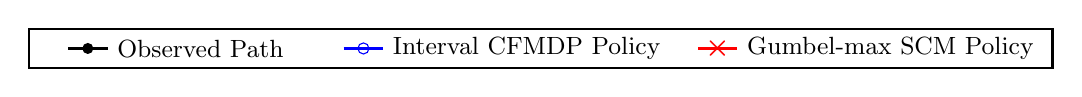
\begin{tikzpicture}[scale=1.0, every node/.style={scale=1.0}]
            \draw[thick, black] (-3, -0.25) rectangle (10, 0.25);
            %
            \draw[black, line width=1pt] (-2.5, 0.0) -- (-2,0.0);
            \fill[black] (-2.25,0.0) circle (2pt); %
            \node[right] at (-2,0.0) {\small Observed Path};
            
            %
            \draw[blue, line width=1pt] (1.0,0.0) -- (1.5,0.0);
            \node[draw=blue, circle, minimum size=4pt, inner sep=0pt] at (1.25,0.0) {}; %
            \node[right] at (1.5,0.0) {\small Interval CFMDP Policy};
            
            %
            \draw[red, line width=1pt] (5.5,0) -- (6,0);
            \node[red] at (5.75,0) {$\boldsymbol{\times}$}; %
            \node[right] at (6,0) {\small Gumbel-max SCM Policy};
        \end{tikzpicture}
    }\\
    %
    \subfigure[\footnotesize Lowest cumulative reward: Interval CFMDP ($312$), Gumbel-max SCM ($312$)]{%
        \resizebox{0.76\columnwidth}{!}{
             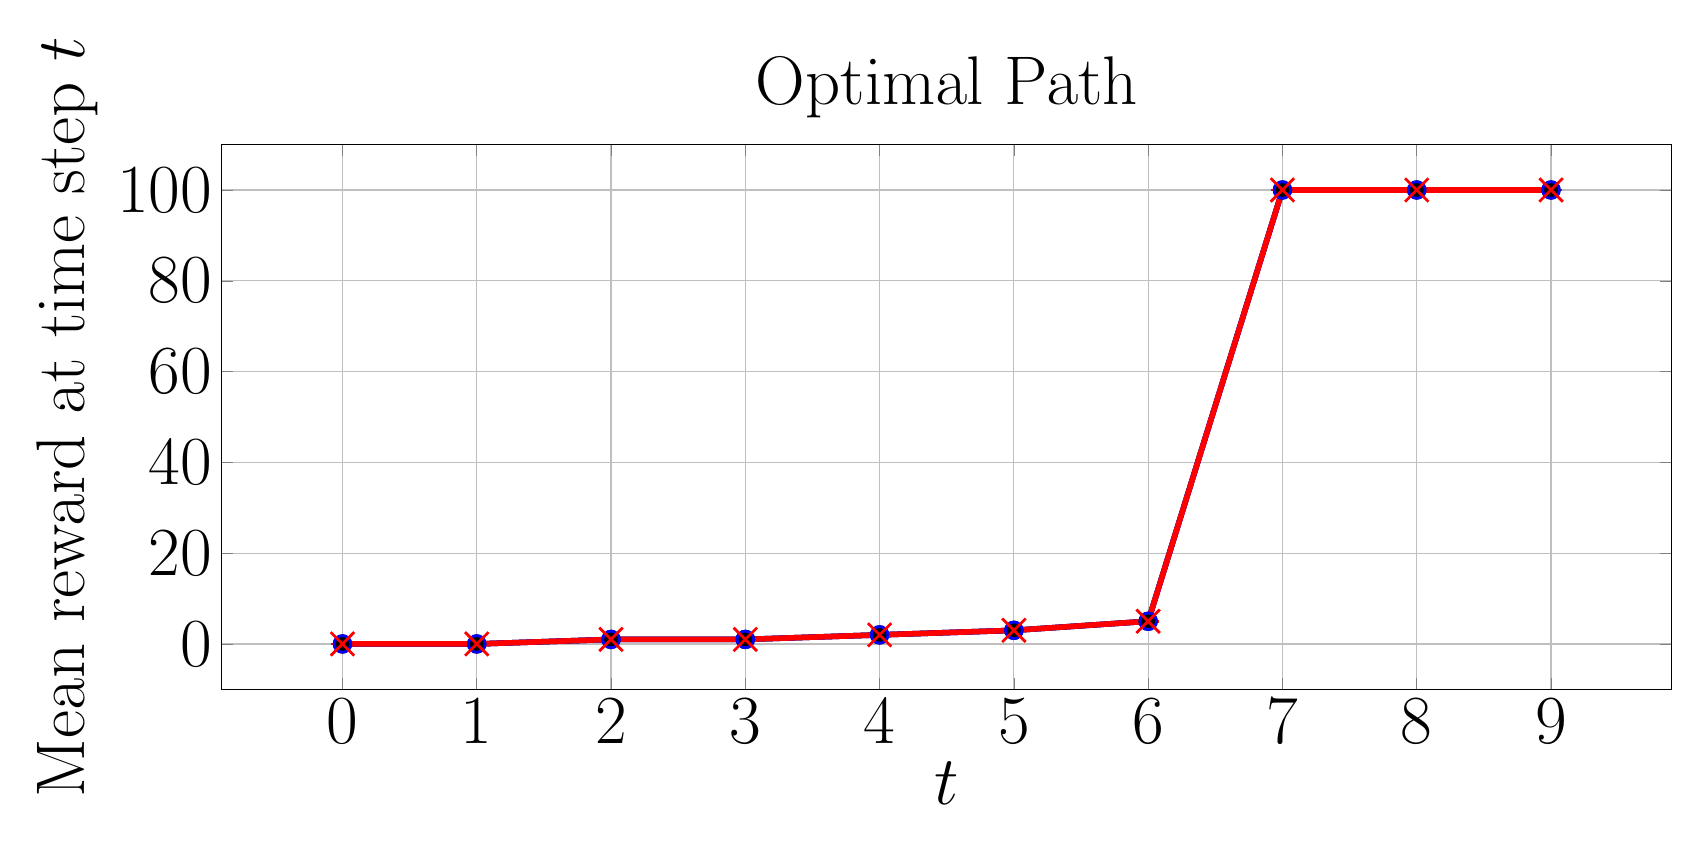
\begin{tikzpicture}
                \begin{axis}[
                    xlabel={$t$},
                    ylabel={Mean reward at time step $t$},
                    title={Optimal Path},
                    grid=both,
                    width=20cm, height=8.5cm,
                    every axis/.style={font=\Huge},
                    %
                ]
                \addplot[
                    color=black, %
                    mark=*, %
                    line width=2pt,
                    mark size=3pt,
                    error bars/.cd,
                    y dir=both, %
                    y explicit, %
                    error bar style={line width=1pt,solid},
                    error mark options={line width=1pt,mark size=4pt,rotate=90}
                ]
                coordinates {
                    (0, 0.0)  +- (0, 0.0)
                    (1, 0.0)  +- (0, 0.0) 
                    (2, 1.0)  +- (0, 0.0) 
                    (3, 1.0)  +- (0, 0.0)
                    (4, 2.0)  +- (0, 0.0)
                    (5, 3.0) +- (0, 0.0)
                    (6, 5.0) +- (0, 0.0)
                    (7, 100.0) +- (0, 0.0)
                    (8, 100.0) +- (0, 0.0)
                    (9, 100.0) +- (0, 0.0)
                };
                %
                \addplot[
                    color=blue, %
                    mark=o, %
                    line width=2pt,
                    mark size=3pt,
                    error bars/.cd,
                    y dir=both, %
                    y explicit, %
                    error bar style={line width=1pt,solid},
                    error mark options={line width=1pt,mark size=4pt,rotate=90}
                ]
                 coordinates {
                    (0, 0.0)  +- (0, 0.0)
                    (1, 0.0)  +- (0, 0.0) 
                    (2, 1.0)  +- (0, 0.0) 
                    (3, 1.0)  +- (0, 0.0)
                    (4, 2.0)  +- (0, 0.0)
                    (5, 3.0) +- (0, 0.0)
                    (6, 5.0) +- (0, 0.0)
                    (7, 100.0) +- (0, 0.0)
                    (8, 100.0) +- (0, 0.0)
                    (9, 100.0) +- (0, 0.0)
                };
                %
                \addplot[
                    color=red, %
                    mark=x, %
                    line width=2pt,
                    mark size=6pt,
                    error bars/.cd,
                    y dir=both, %
                    y explicit, %
                    error bar style={line width=1pt,solid},
                    error mark options={line width=1pt,mark size=4pt,rotate=90}
                ]
                coordinates {
                    (0, 0.0)  +- (0, 0.0)
                    (1, 0.0)  +- (0, 0.0) 
                    (2, 1.0)  +- (0, 0.0) 
                    (3, 1.0)  +- (0, 0.0)
                    (4, 2.0)  +- (0, 0.0)
                    (5, 3.0) +- (0, 0.0)
                    (6, 5.0) +- (0, 0.0)
                    (7, 100.0) +- (0, 0.0)
                    (8, 100.0) +- (0, 0.0)
                    (9, 100.0) +- (0, 0.0)
                };
                \end{axis}
            \end{tikzpicture}
         }
    }
    \hspace{1cm}
    \subfigure[\footnotesize Lowest cumulative reward: Interval CFMDP ($19$), Gumbel-max SCM ($-88$)]{%
         \resizebox{0.76\columnwidth}{!}{
            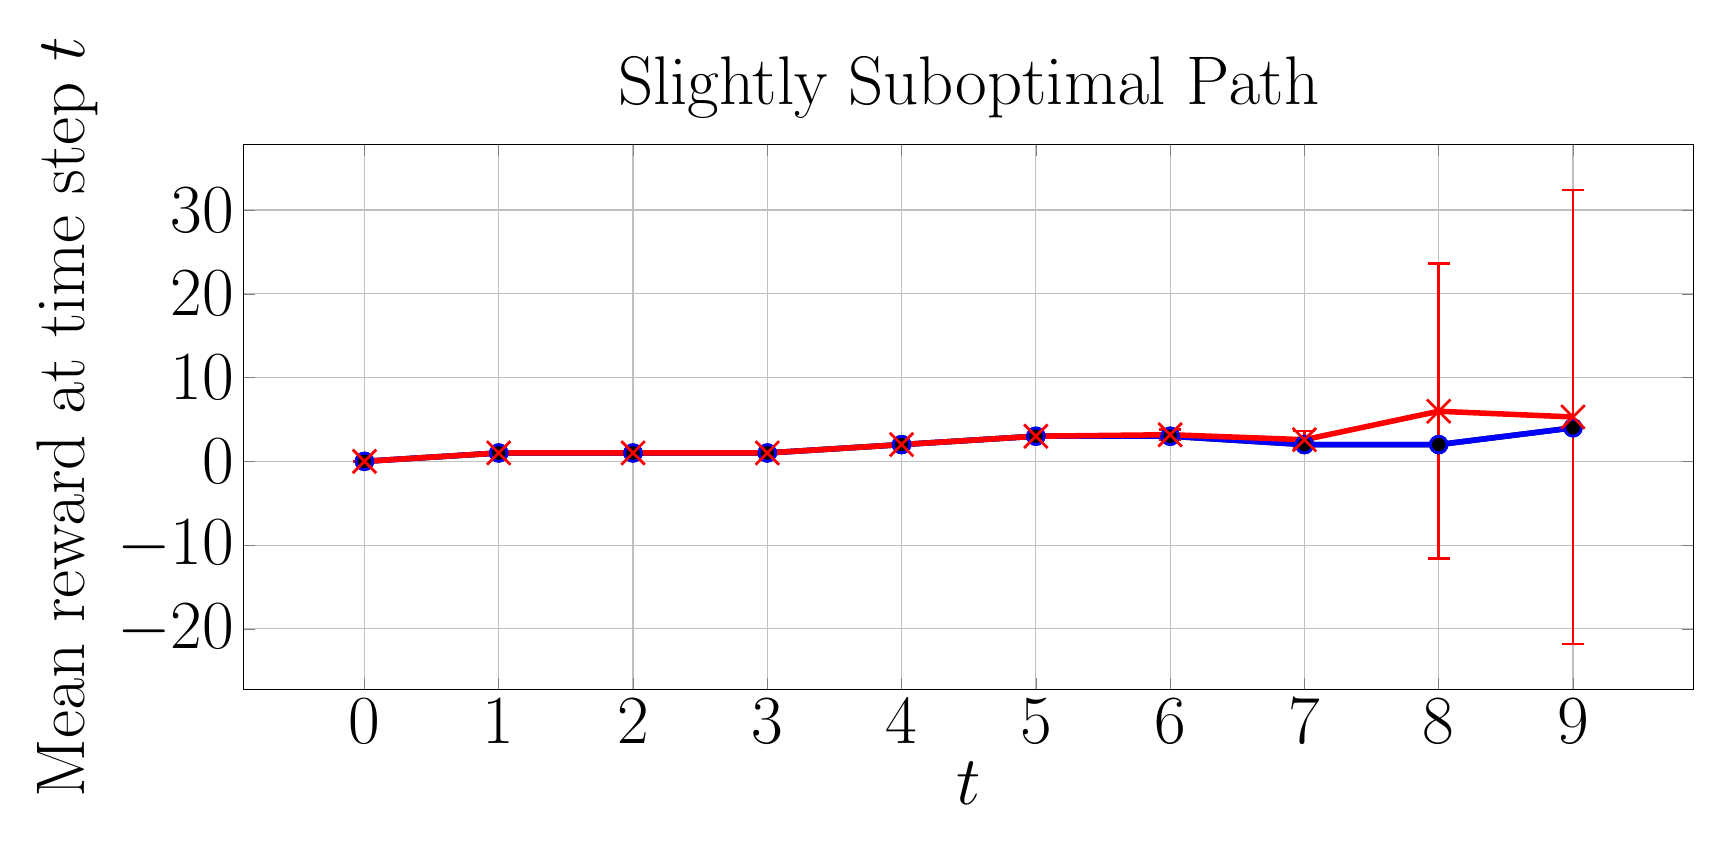
\begin{tikzpicture}
                \begin{axis}[
                    xlabel={$t$},
                    ylabel={Mean reward at time step $t$},
                    title={Slightly Suboptimal Path},
                    grid=both,
                    width=20cm, height=8.5cm,
                    every axis/.style={font=\Huge},
                    %
                ]
                \addplot[
                    color=black, %
                    mark=*, %
                    line width=2pt,
                    mark size=3pt,
                    error bars/.cd,
                    y dir=both, %
                    y explicit, %
                    error bar style={line width=1pt,solid},
                    error mark options={line width=1pt,mark size=4pt,rotate=90}
                ]
              coordinates {
                    (0, 0.0)  +- (0, 0.0)
                    (1, 1.0)  +- (0, 0.0) 
                    (2, 1.0)  +- (0, 0.0) 
                    (3, 1.0)  +- (0, 0.0)
                    (4, 2.0)  +- (0, 0.0)
                    (5, 3.0) +- (0, 0.0)
                    (6, 3.0) +- (0, 0.0)
                    (7, 2.0) +- (0, 0.0)
                    (8, 2.0) +- (0, 0.0)
                    (9, 4.0) +- (0, 0.0)
                };
                %
                \addplot[
                    color=blue, %
                    mark=o, %
                    line width=2pt,
                    mark size=3pt,
                    error bars/.cd,
                    y dir=both, %
                    y explicit, %
                    error bar style={line width=1pt,solid},
                    error mark options={line width=1pt,mark size=4pt,rotate=90}
                ]
              coordinates {
                    (0, 0.0)  +- (0, 0.0)
                    (1, 1.0)  +- (0, 0.0) 
                    (2, 1.0)  +- (0, 0.0) 
                    (3, 1.0)  +- (0, 0.0)
                    (4, 2.0)  +- (0, 0.0)
                    (5, 3.0) +- (0, 0.0)
                    (6, 3.0) +- (0, 0.0)
                    (7, 2.0) +- (0, 0.0)
                    (8, 2.0) +- (0, 0.0)
                    (9, 4.0) +- (0, 0.0)
                };
                %
                \addplot[
                    color=red, %
                    mark=x, %
                    line width=2pt,
                    mark size=6pt,
                    error bars/.cd,
                    y dir=both, %
                    y explicit, %
                    error bar style={line width=1pt,solid},
                    error mark options={line width=1pt,mark size=4pt,rotate=90}
                ]
                coordinates {
                    (0, 0.0)  +- (0, 0.0)
                    (1, 1.0)  +- (0, 0.0) 
                    (2, 1.0)  +- (0, 0.0) 
                    (3, 1.0)  +- (0, 0.0)
                    (4, 2.0)  += (0, 0.0)
                    (5, 3.0)  += (0, 0.0)
                    (6, 3.17847) += (0, 0.62606746) -= (0, 0.62606746)
                    (7, 2.5832885) += (0, 1.04598233) -= (0, 1.04598233)
                    (8, 5.978909) += (0, 17.60137623) -= (0, 17.60137623)
                    (9, 5.297059) += (0, 27.09227512) -= (0, 27.09227512)
                };
                \end{axis}
            \end{tikzpicture}
         }
    }\\[-1.5pt]
    \subfigure[\footnotesize Lowest cumulative reward: Interval CFMDP ($14$), Gumbel-max SCM ($-598$)]{%
         \resizebox{0.76\columnwidth}{!}{
             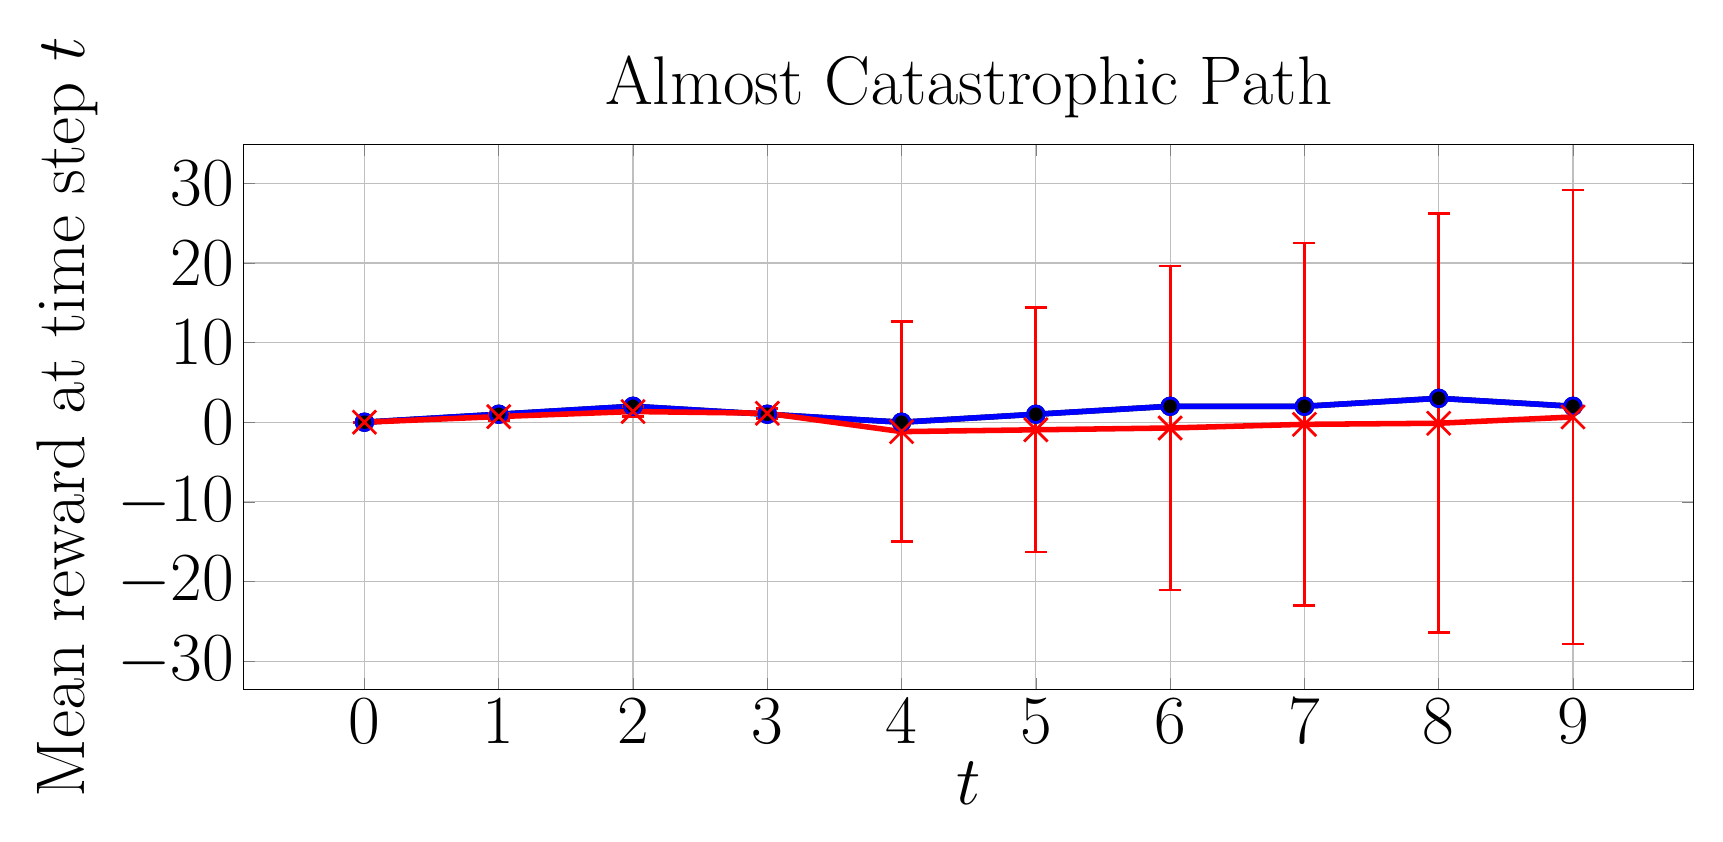
\begin{tikzpicture}
                \begin{axis}[
                    xlabel={$t$},
                    ylabel={Mean reward at time step $t$},
                    title={Almost Catastrophic Path},
                    grid=both,
                    width=20cm, height=8.5cm,
                    every axis/.style={font=\Huge},
                    %
                ]
                \addplot[
                    color=black, %
                    mark=*, %
                    line width=2pt,
                    mark size=3pt,
                    error bars/.cd,
                    y dir=both, %
                    y explicit, %
                    error bar style={line width=1pt,solid},
                    error mark options={line width=1pt,mark size=4pt,rotate=90}
                ]
                coordinates {
                    (0, 0.0)  +- (0, 0.0)
                    (1, 1.0)  +- (0, 0.0) 
                    (2, 2.0)  +- (0, 0.0) 
                    (3, 1.0)  +- (0, 0.0)
                    (4, 0.0)  +- (0, 0.0)
                    (5, 1.0) +- (0, 0.0)
                    (6, 2.0) +- (0, 0.0)
                    (7, 2.0) +- (0, 0.0)
                    (8, 3.0) +- (0, 0.0)
                    (9, 2.0) +- (0, 0.0)
                };
                %
                \addplot[
                    color=blue, %
                    mark=o, %
                    line width=2pt,
                    mark size=3pt,
                    error bars/.cd,
                    y dir=both, %
                    y explicit, %
                    error bar style={line width=1pt,solid},
                    error mark options={line width=1pt,mark size=4pt,rotate=90}
                ]
                coordinates {
                    (0, 0.0)  +- (0, 0.0)
                    (1, 1.0)  +- (0, 0.0) 
                    (2, 2.0)  +- (0, 0.0) 
                    (3, 1.0)  +- (0, 0.0)
                    (4, 0.0)  +- (0, 0.0)
                    (5, 1.0) +- (0, 0.0)
                    (6, 2.0) +- (0, 0.0)
                    (7, 2.0) +- (0, 0.0)
                    (8, 3.0) +- (0, 0.0)
                    (9, 2.0) +- (0, 0.0)
                };
                %
                \addplot[
                    color=red, %
                    mark=x, %
                    line width=2pt,
                    mark size=6pt,
                    error bars/.cd,
                    y dir=both, %
                    y explicit, %
                    error bar style={line width=1pt,solid},
                    error mark options={line width=1pt,mark size=4pt,rotate=90}
                ]
                coordinates {
                    (0, 0.0)  +- (0, 0.0)
                    (1, 0.7065655)  +- (0, 0.4553358) 
                    (2, 1.341673)  +- (0, 0.67091621) 
                    (3, 1.122926)  +- (0, 0.61281824)
                    (4, -1.1821935)  +- (0, 13.82444042)
                    (5, -0.952399)  +- (0, 15.35195457)
                    (6, -0.72672) +- (0, 20.33508414)
                    (7, -0.268983) +- (0, 22.77861454)
                    (8, -0.1310835) +- (0, 26.31013314)
                    (9, 0.65806) +- (0, 28.50670214)
                };
                %
            %
            %
            %
            %
            %
            %
            %
            %
            %
            %
            %
            %
            %
            %
            %
            %
            %
            %
                \end{axis}
            \end{tikzpicture}
         }
    }
    \hspace{1cm}
    \subfigure[\footnotesize Lowest cumulative reward: Interval CFMDP ($-698$), Gumbel-max SCM ($-698$)]{%
         \resizebox{0.76\columnwidth}{!}{
            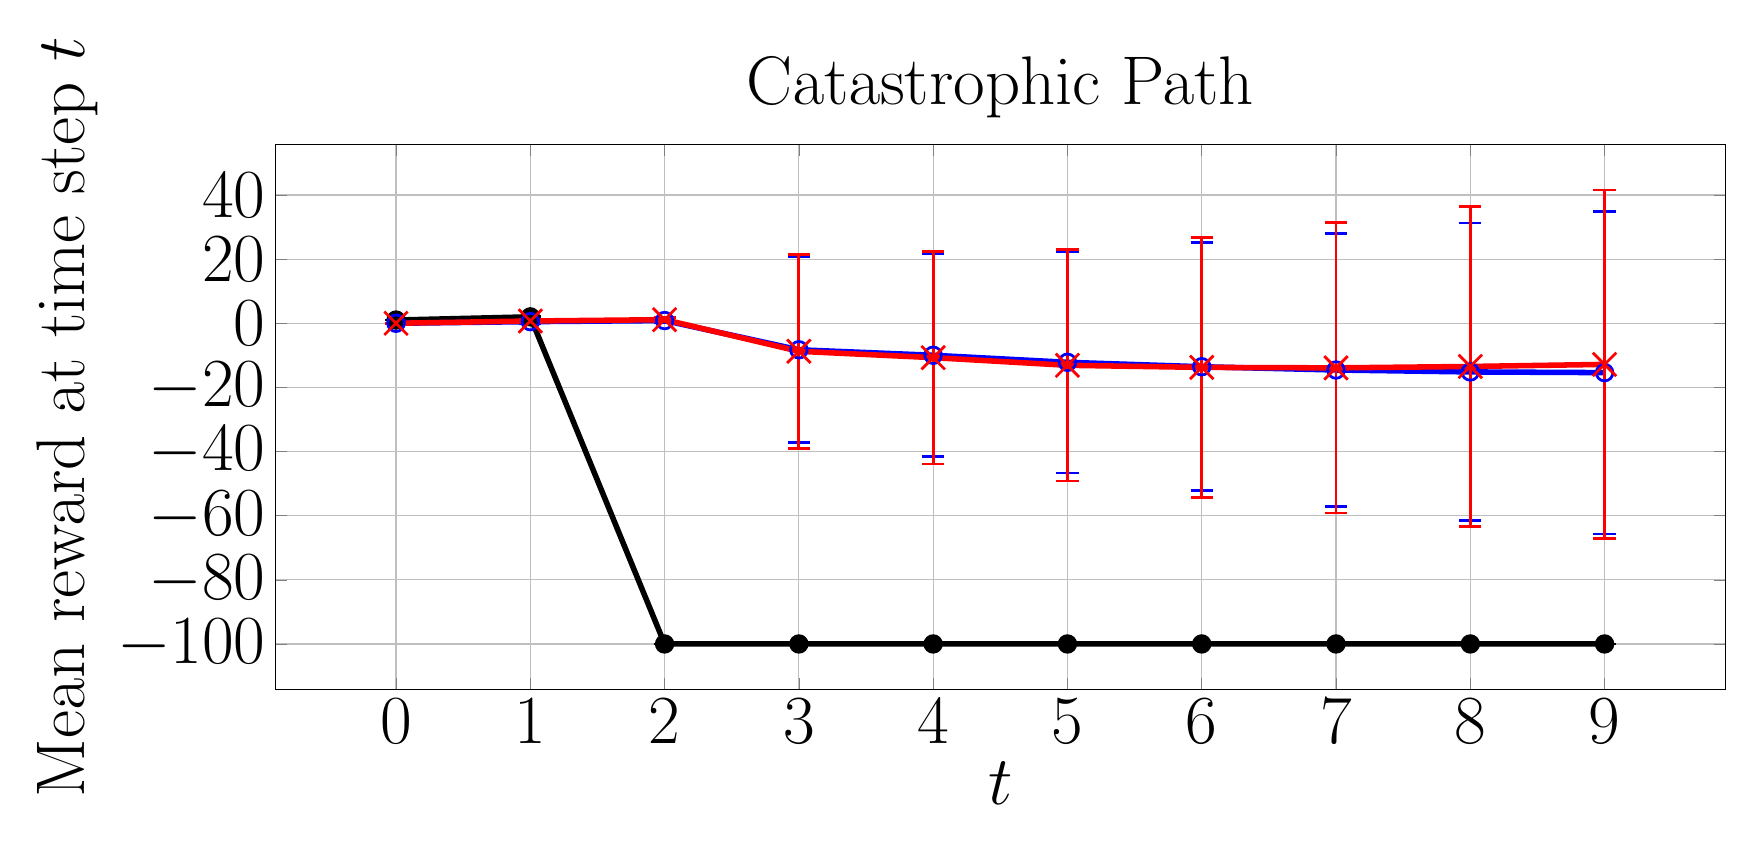
\begin{tikzpicture}
                \begin{axis}[
                    xlabel={$t$},
                    ylabel={Mean reward at time step $t$},
                    title={Catastrophic Path},
                    grid=both,
                    width=20cm, height=8.5cm,
                    every axis/.style={font=\Huge},
                    %
                ]
                \addplot[
                    color=black, %
                    mark=*, %
                    line width=2pt,
                    mark size=3pt,
                    error bars/.cd,
                    y dir=both, %
                    y explicit, %
                    error bar style={line width=1pt,solid},
                    error mark options={line width=1pt,mark size=4pt,rotate=90}
                ]
                coordinates {
                    (0, 1.0)  +- (0, 0.0)
                    (1, 2.0)  +- (0, 0.0) 
                    (2, -100.0)  +- (0, 0.0) 
                    (3, -100.0)  +- (0, 0.0)
                    (4, -100.0)  +- (0, 0.0)
                    (5, -100.0) +- (0, 0.0)
                    (6, -100.0) +- (0, 0.0)
                    (7, -100.0) +- (0, 0.0)
                    (8, -100.0) +- (0, 0.0)
                    (9, -100.0) +- (0, 0.0)
                };
                %
                \addplot[
                    color=blue, %
                    mark=o, %
                    line width=2pt,
                    mark size=3pt,
                    error bars/.cd,
                    y dir=both, %
                    y explicit, %
                    error bar style={line width=1pt,solid},
                    error mark options={line width=1pt,mark size=4pt,rotate=90}
                ]
                coordinates {
                    (0, 0.0)  +- (0, 0.0)
                    (1, 0.504814)  +- (0, 0.49997682) 
                    (2, 0.8439835)  +- (0, 0.76831917) 
                    (3, -8.2709165)  +- (0, 28.93656754)
                    (4, -9.981082)  +- (0, 31.66825363)
                    (5, -12.1776325) +- (0, 34.53463233)
                    (6, -13.556076) +- (0, 38.62845372)
                    (7, -14.574418) +- (0, 42.49603359)
                    (8, -15.1757075) +- (0, 46.41913968)
                    (9, -15.3900395) +- (0, 50.33563368)
                };
                %
                \addplot[
                    color=red, %
                    mark=x, %
                    line width=2pt,
                    mark size=6pt,
                    error bars/.cd,
                    y dir=both, %
                    y explicit, %
                    error bar style={line width=1pt,solid},
                    error mark options={line width=1pt,mark size=4pt,rotate=90}
                ]
                coordinates {
                    (0, 0.0)  +- (0, 0.0)
                    (1, 0.701873)  +- (0, 0.45743556) 
                    (2, 1.1227805)  +- (0, 0.73433129) 
                    (3, -8.7503255)  +- (0, 30.30257976)
                    (4, -10.722092)  +- (0, 33.17618589)
                    (5, -13.10721)  +- (0, 36.0648089)
                    (6, -13.7631645) +- (0, 40.56553451)
                    (7, -13.909043) +- (0, 45.23829402)
                    (8, -13.472517) +- (0, 49.96270296)
                    (9, -12.8278835) +- (0, 54.38618735)
                };
                %
            %
            %
            %
            %
            %
            %
            %
            %
            %
            %
            %
            %
            %
            %
            %
            %
            %
            %
                \end{axis}
            \end{tikzpicture}
         }
    }
    \caption{Average instant reward of CF paths induced by policies on GridWorld $p=0.4$.}
    \label{fig: reward p=0.4}
\end{figure*}

\subsection{Experimental Setup}
To compare policy performance, we measure the average rewards of counterfactual paths induced by our policy and the Gumbel-max policy by uniformly sampling $200$ counterfactual MDPs from the ICFMDP and generating $10,000$ counterfactual paths over each sampled CFMDP. \jl{Since the interval CFMDP depends on the observed path, we select $4$  paths of varying optimality to evaluate how the observed path impacts the performance of both policies: an optimal path, a slightly suboptimal path that could reach the optimal reward with a few changes, a catastrophic path that enters a catastrophic, terminal state with low reward, and an almost catastrophic path that was close to entering a catastrophic state.} When measuring the average probability bound widths and execution time needed to generate the ICFMDPs, we averaged over $20$ randomly generated observed paths
\footnote{Further training details are provided in Appendix \ref{app: training details}, and the code is provided at \href{https://github.com/ddv-lab/robust-cf-inference-in-MDPs}{https://github.com/ddv-lab/robust-cf-inference-in-MDPs}
%
%
.}.

\subsection{GridWorld}
\jl{The GridWorld MDP is a $4 \times 4$ grid where an agent must navigate from the top-left corner to the goal state in the bottom-right corner, avoiding a dangerous terminal state in the centre. At each time step, the agent can move up, down, left, or right, but there is a small probability (controlled by hyper-parameter $p$) of moving in an unintended direction. As the agent nears the goal, the reward for each state increases, culminating in a reward of $+100$ for reaching the goal. Entering the dangerous state results in a penalty of $-100$. We use two versions of GridWorld: a less stochastic version with $p=0.9$ (i.e., $90$\% chance of moving in the chosen direction) and a more stochastic version with $p=0.4$.}

\paragraph{GridWorld ($p=0.9$)}
When $p=0.9$, the counterfactual probability bounds are typically narrow (see Table \ref{tab:nonzero_probs} for average measurements). Consequently, as shown in Figure \ref{fig: reward p=0.9}, both policies are nearly identical and perform similarly well across the optimal, slightly suboptimal, and catastrophic paths.
%
However, for the almost catastrophic path, the interval CFMDP path is more conservative and follows the observed path more closely (as this is where the probability bounds are narrowest), which typically requires one additional step to reach the goal state than the Gumbel-max SCM policy.
%

\paragraph{GridWorld ($p=0.4$)}
\jl{When $p=0.4$, the GridWorld environment becomes more uncertain, increasing the risk of entering the dangerous state even if correct actions are chosen. Thus, as shown in Figure \ref{fig: reward p=0.4}, the interval CFMDP policy adopts a more conservative approach, avoiding deviation from the observed policy if it cannot guarantee higher counterfactual rewards (see the slightly suboptimal and almost catastrophic paths), whereas the Gumbel-max SCM is inconsistent: it can yield higher rewards, but also much lower rewards, reflected in the wide error bars.} For the catastrophic path, both policies must deviate from the observed path to achieve a higher reward and, in this case, perform similarly.
%
%
%
%
\subsection{Sepsis}
The Sepsis MDP \citep{oberst2019counterfactual} simulates trajectories of Sepsis patients. Each state consists of four vital signs (heart rate, blood pressure, oxygen concentration, and glucose levels), categorised as low, normal, or high.
and three treatments that can be toggled on/off at each time step (8 actions in total). Unlike \citet{oberst2019counterfactual}, we scale rewards based on the number of out-of-range vital signs, between $-1000$ (patient dies) and $1000$ (patient discharged). \jl{Like the GridWorld $p=0.4$ experiment, the Sepsis MDP is highly uncertain, as many states are equally likely to lead to optimal and poor outcomes. Thus, as shown in Figure \ref{fig: reward sepsis}, both policies follow the observed optimal and almost catastrophic paths to guarantee rewards are no worse than the observation.} However, improving the catastrophic path requires deviating from the observation. Here, the Gumbel-max SCM policy, on average, performs better than the interval CFMDP policy. But, since both policies have lower bounds clipped at $-1000$, neither policy reliably improves over the observation. In contrast, for the slightly suboptimal path, the interval CFMDP policy performs significantly better, shown by its higher lower bounds. 
Moreover, in these two cases, the worst-case counterfactual path generated by the interval CFMDP policy is better than that of the Gumbel-max SCM policy,
indicating its greater robustness.
%
\begin{figure*}
    \centering
     \resizebox{0.6\textwidth}{!}{
        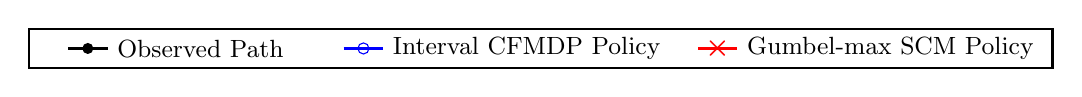
\begin{tikzpicture}[scale=1.0, every node/.style={scale=1.0}]
            \draw[thick, black] (-3, -0.25) rectangle (10, 0.25);
            %
            \draw[black, line width=1pt] (-2.5, 0.0) -- (-2,0.0);
            \fill[black] (-2.25,0.0) circle (2pt); %
            \node[right] at (-2,0.0) {\small Observed Path};
            
            %
            \draw[blue, line width=1pt] (1.0,0.0) -- (1.5,0.0);
            \node[draw=blue, circle, minimum size=4pt, inner sep=0pt] at (1.25,0.0) {}; %
            \node[right] at (1.5,0.0) {\small Interval CFMDP Policy};
            
            %
            \draw[red, line width=1pt] (5.5,0) -- (6,0);
            \node[red] at (5.75,0) {$\boldsymbol{\times}$}; %
            \node[right] at (6,0) {\small Gumbel-max SCM Policy};
        \end{tikzpicture}
    }\\
    \subfigure[\footnotesize Lowest cumulative reward: Interval CFMDP ($8000$), Gumbel-max SCM ($8000$)]{%
         \resizebox{0.76\columnwidth}{!}{
             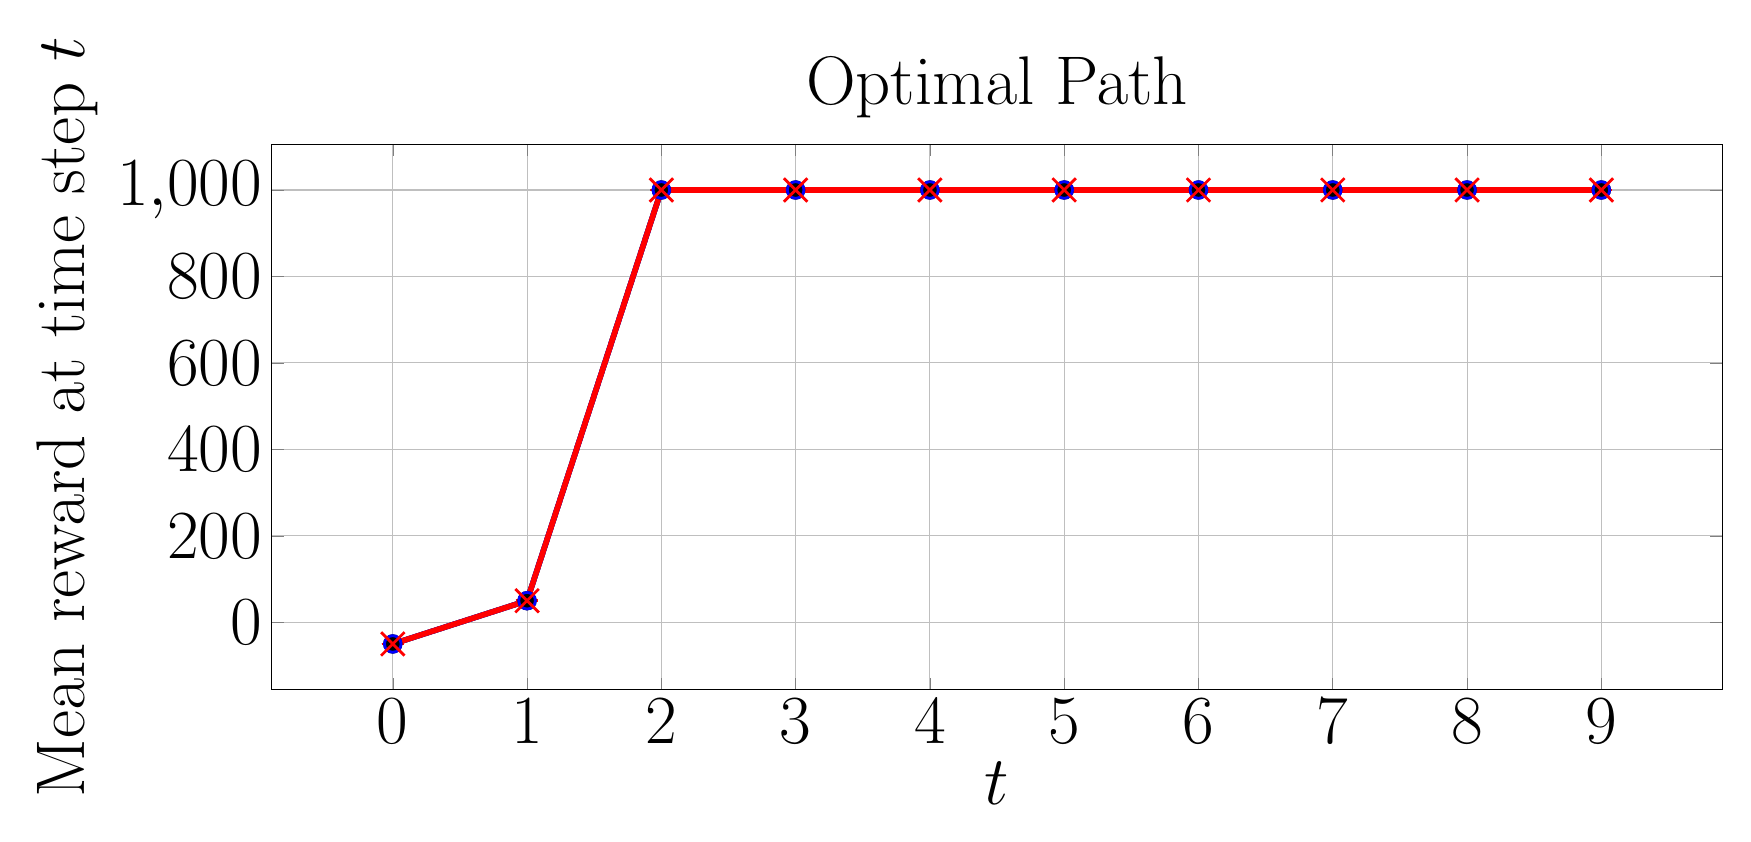
\begin{tikzpicture}
                \begin{axis}[
                    xlabel={$t$},
                    ylabel={Mean reward at time step $t$},
                    title={Optimal Path},
                    grid=both,
                    width=20cm, height=8.5cm,
                    every axis/.style={font=\Huge},
                    %
                ]
                \addplot[
                    color=black, %
                    mark=*, %
                    line width=2pt,
                    mark size=3pt,
                ]
                coordinates {
                    (0, -50.0)
                    (1, 50.0)
                    (2, 1000.0)
                    (3, 1000.0)
                    (4, 1000.0)
                    (5, 1000.0)
                    (6, 1000.0)
                    (7, 1000.0)
                    (8, 1000.0)
                    (9, 1000.0)
                };
                %
                \addplot[
                    color=blue, %
                    mark=o, %
                    line width=2pt,
                    mark size=3pt,
                    error bars/.cd,
                    y dir=both, %
                    y explicit, %
                    error bar style={line width=1pt,solid},
                    error mark options={line width=1pt,mark size=4pt,rotate=90}
                ]
                coordinates {
                    (0, -50.0)  +- (0, 0.0)
                    (1, 50.0)  +- (0, 0.0) 
                    (2, 1000.0)  +- (0, 0.0) 
                    (3, 1000.0)  +- (0, 0.0)
                    (4, 1000.0)  +- (0, 0.0)
                    (5, 1000.0) +- (0, 0.0)
                    (6, 1000.0) +- (0, 0.0)
                    (7, 1000.0) +- (0, 0.0)
                    (8, 1000.0) +- (0, 0.0)
                    (9, 1000.0) +- (0, 0.0)
                };
                %
                \addplot[
                    color=red, %
                    mark=x, %
                    line width=2pt,
                    mark size=6pt,
                    error bars/.cd,
                    y dir=both, %
                    y explicit, %
                    error bar style={line width=1pt,solid},
                    error mark options={line width=1pt,mark size=4pt,rotate=90}
                ]
                coordinates {
                    (0, -50.0)  +- (0, 0.0)
                    (1, 50.0)  +- (0, 0.0) 
                    (2, 1000.0)  +- (0, 0.0) 
                    (3, 1000.0)  +- (0, 0.0)
                    (4, 1000.0)  +- (0, 0.0)
                    (5, 1000.0) +- (0, 0.0)
                    (6, 1000.0) +- (0, 0.0)
                    (7, 1000.0) +- (0, 0.0)
                    (8, 1000.0) +- (0, 0.0)
                    (9, 1000.0) +- (0, 0.0)
                };
                %
                \end{axis}
            \end{tikzpicture}
         }
    }
    \hspace{1cm}
    \subfigure[\footnotesize Lowest cumulative reward: Interval CFMDP ($-5980$), Gumbel-max SCM ($-8000$)]{%
         \resizebox{0.76\columnwidth}{!}{
            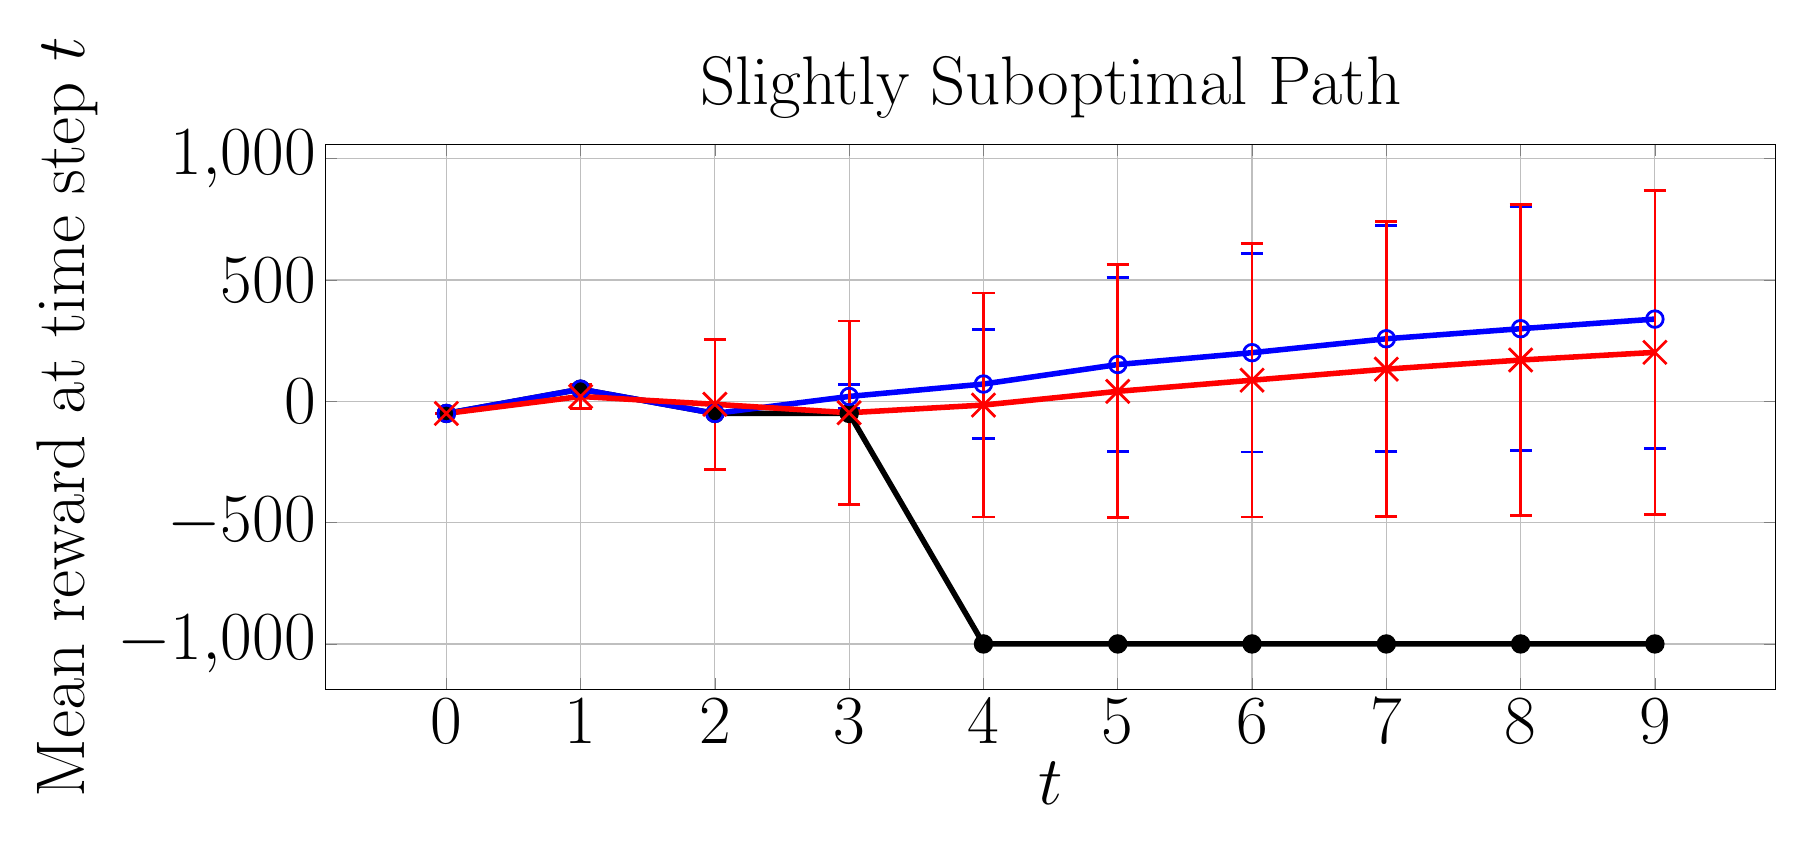
\begin{tikzpicture}
                \begin{axis}[
                    xlabel={$t$},
                    ylabel={Mean reward at time step $t$},
                    title={Slightly Suboptimal Path},
                    grid=both,
                    width=20cm, height=8.5cm,
                    every axis/.style={font=\Huge},
                    %
                ]
               \addplot[
                    color=black, %
                    mark=*, %
                    line width=2pt,
                    mark size=3pt,
                ]
                coordinates {
                    (0, -50.0)
                    (1, 50.0)
                    (2, -50.0)
                    (3, -50.0)
                    (4, -1000.0)
                    (5, -1000.0)
                    (6, -1000.0)
                    (7, -1000.0)
                    (8, -1000.0)
                    (9, -1000.0)
                };
                %
                \addplot[
                    color=blue, %
                    mark=o, %
                    line width=2pt,
                    mark size=3pt,
                    error bars/.cd,
                    y dir=both, %
                    y explicit, %
                    error bar style={line width=1pt,solid},
                    error mark options={line width=1pt,mark size=4pt,rotate=90}
                ]
                coordinates {
                    (0, -50.0)  +- (0, 0.0)
                    (1, 50.0)  +- (0, 0.0) 
                    (2, -50.0)  +- (0, 0.0) 
                    (3, 20.0631)  +- (0, 49.97539413)
                    (4, 71.206585)  +- (0, 226.02033693)
                    (5, 151.60797) +- (0, 359.23292559)
                    (6, 200.40593) +- (0, 408.86185176)
                    (7, 257.77948) +- (0, 466.10372804)
                    (8, 299.237465) +- (0, 501.82579506)
                    (9, 338.9129) +- (0, 532.06124996)
                };
                %
                \addplot[
                    color=red, %
                    mark=x, %
                    line width=2pt,
                    mark size=6pt,
                    error bars/.cd,
                    y dir=both, %
                    y explicit, %
                    error bar style={line width=1pt,solid},
                    error mark options={line width=1pt,mark size=4pt,rotate=90}
                ]
                coordinates {
                    (0, -50.0)  +- (0, 0.0)
                    (1, 20.00736)  +- (0, 49.99786741) 
                    (2, -12.282865)  +- (0, 267.598755) 
                    (3, -47.125995)  +- (0, 378.41755832)
                    (4, -15.381965)  +- (0, 461.77616558)
                    (5, 41.15459) +- (0, 521.53189262)
                    (6, 87.01595) +- (0, 564.22243126 )
                    (7, 132.62376) +- (0, 607.31338037)
                    (8, 170.168145) +- (0, 641.48013693)
                    (9, 201.813135) +- (0, 667.29441777)
                };
                %
                %
                %
                %
                %
                %
                %
                %
                %
                %
                %
                %
                %
                %
                %
                %
                %
                %
                %
                \end{axis}
            \end{tikzpicture}
         }
    }\\[-1.5pt]
    \subfigure[\footnotesize Lowest cumulative reward: Interval CFMDP ($100$), Gumbel-max SCM ($100$)]{%
         \resizebox{0.76\columnwidth}{!}{
             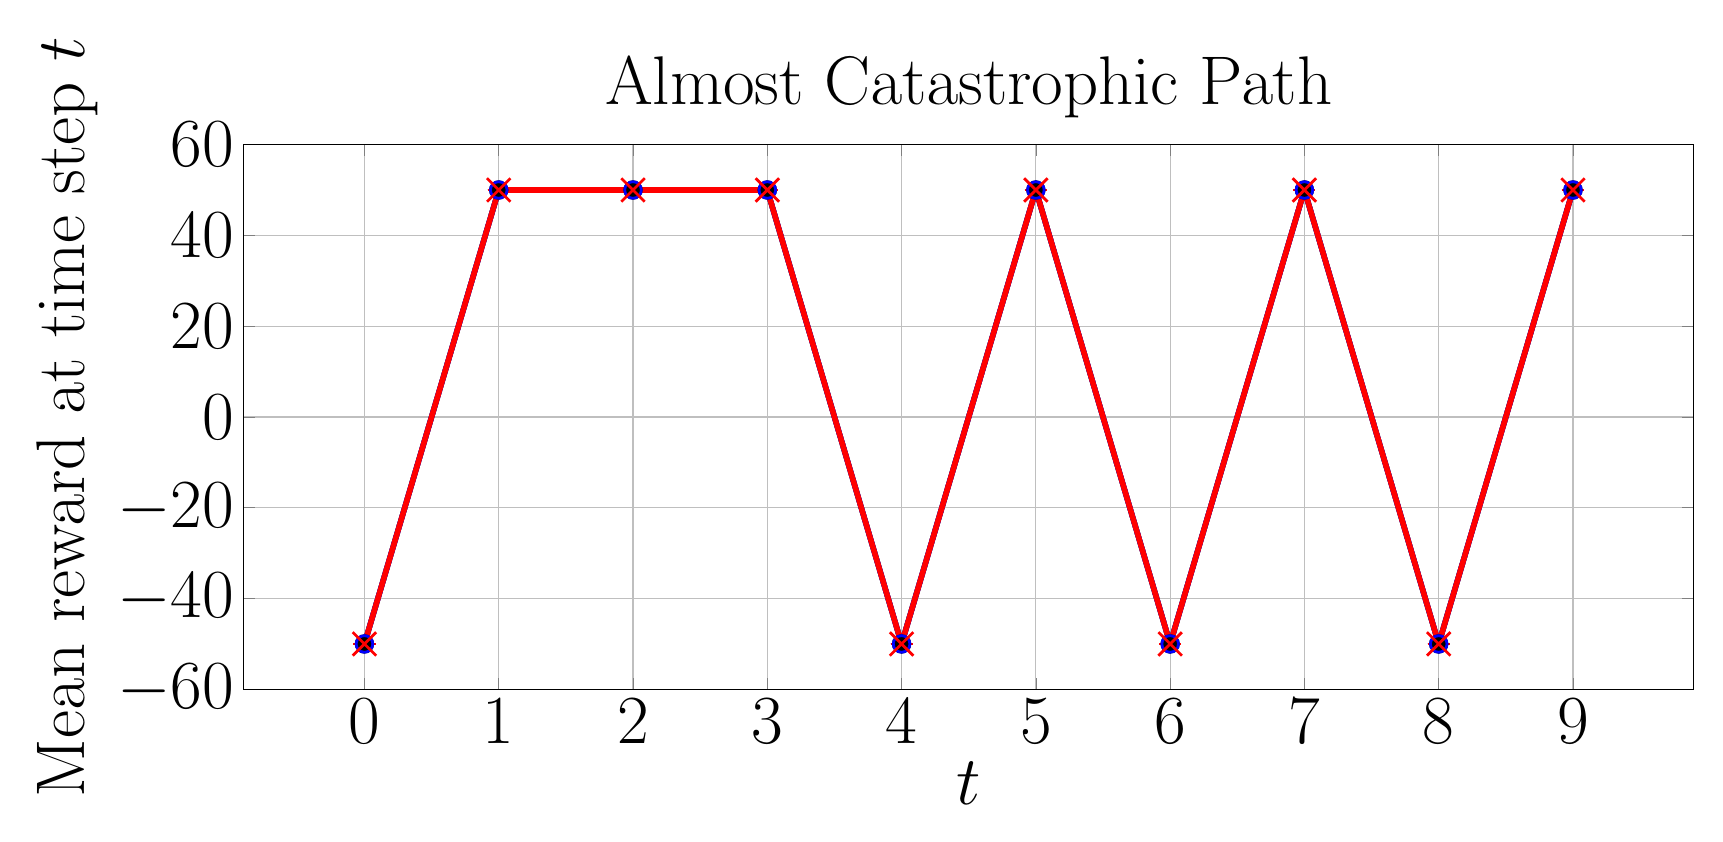
\begin{tikzpicture}
                \begin{axis}[
                    xlabel={$t$},
                    ylabel={Mean reward at time step $t$},
                    title={Almost Catastrophic Path},
                    grid=both,
                    every axis/.style={font=\Huge},
                    width=20cm, height=8.5cm,
                    %
                ]
               \addplot[
                    color=black, %
                    mark=*, %
                    line width=2pt,
                    mark size=3pt,
                ]
                coordinates {
                    (0, -50.0)
                    (1, 50.0)
                    (2, 50.0)
                    (3, 50.0)
                    (4, -50.0)
                    (5, 50.0)
                    (6, -50.0)
                    (7, 50.0)
                    (8, -50.0)
                    (9, 50.0)
                };
                %
                %
                \addplot[
                    color=blue, %
                    mark=o, %
                    line width=2pt,
                    mark size=3pt,
                    error bars/.cd,
                    y dir=both, %
                    y explicit, %
                    error bar style={line width=1pt,solid},
                    error mark options={line width=1pt,mark size=4pt,rotate=90}
                ]
                coordinates {
                    (0, -50.0)  +- (0, 0.0)
                    (1, 50.0)  +- (0, 0.0) 
                    (2, 50.0)  +- (0, 0.0) 
                    (3, 50.0)  +- (0, 0.0)
                    (4, -50.0)  +- (0, 0.0)
                    (5, 50.0) +- (0, 0.0)
                    (6, -50.0) +- (0, 0.0)
                    (7, 50.0) +- (0, 0.0)
                    (8, -50.0) +- (0, 0.0)
                    (9, 50.0) +- (0, 0.0)
                };
                %
                \addplot[
                    color=red, %
                    mark=x, %
                    line width=2pt,
                    mark size=6pt,
                    error bars/.cd,
                    y dir=both, %
                    y explicit, %
                    error bar style={line width=1pt,solid},
                    error mark options={line width=1pt,mark size=4pt,rotate=90}
                ]
                coordinates {
                    (0, -50.0)  +- (0, 0.0)
                    (1, 50.0)  +- (0, 0.0) 
                    (2, 50.0)  +- (0, 0.0) 
                    (3, 50.0)  +- (0, 0.0)
                    (4, -50.0)  +- (0, 0.0)
                    (5, 50.0) +- (0, 0.0)
                    (6, -50.0) +- (0, 0.0)
                    (7, 50.0) +- (0, 0.0)
                    (8, -50.0) +- (0, 0.0)
                    (9, 50.0) +- (0, 0.0)
                };
                %
                %
                %
                %
                %
                %
                %
                %
                %
                %
                %
                %
                %
                %
                %
                %
                %
                %
                %
                \end{axis}
            \end{tikzpicture}
         }
    }
    \hspace{1cm}
    \subfigure[\footnotesize Lowest cumulative reward: Interval CFMDP ($-7150$), Gumbel-max SCM ($-9050$)]{%
         \resizebox{0.76\columnwidth}{!}{
            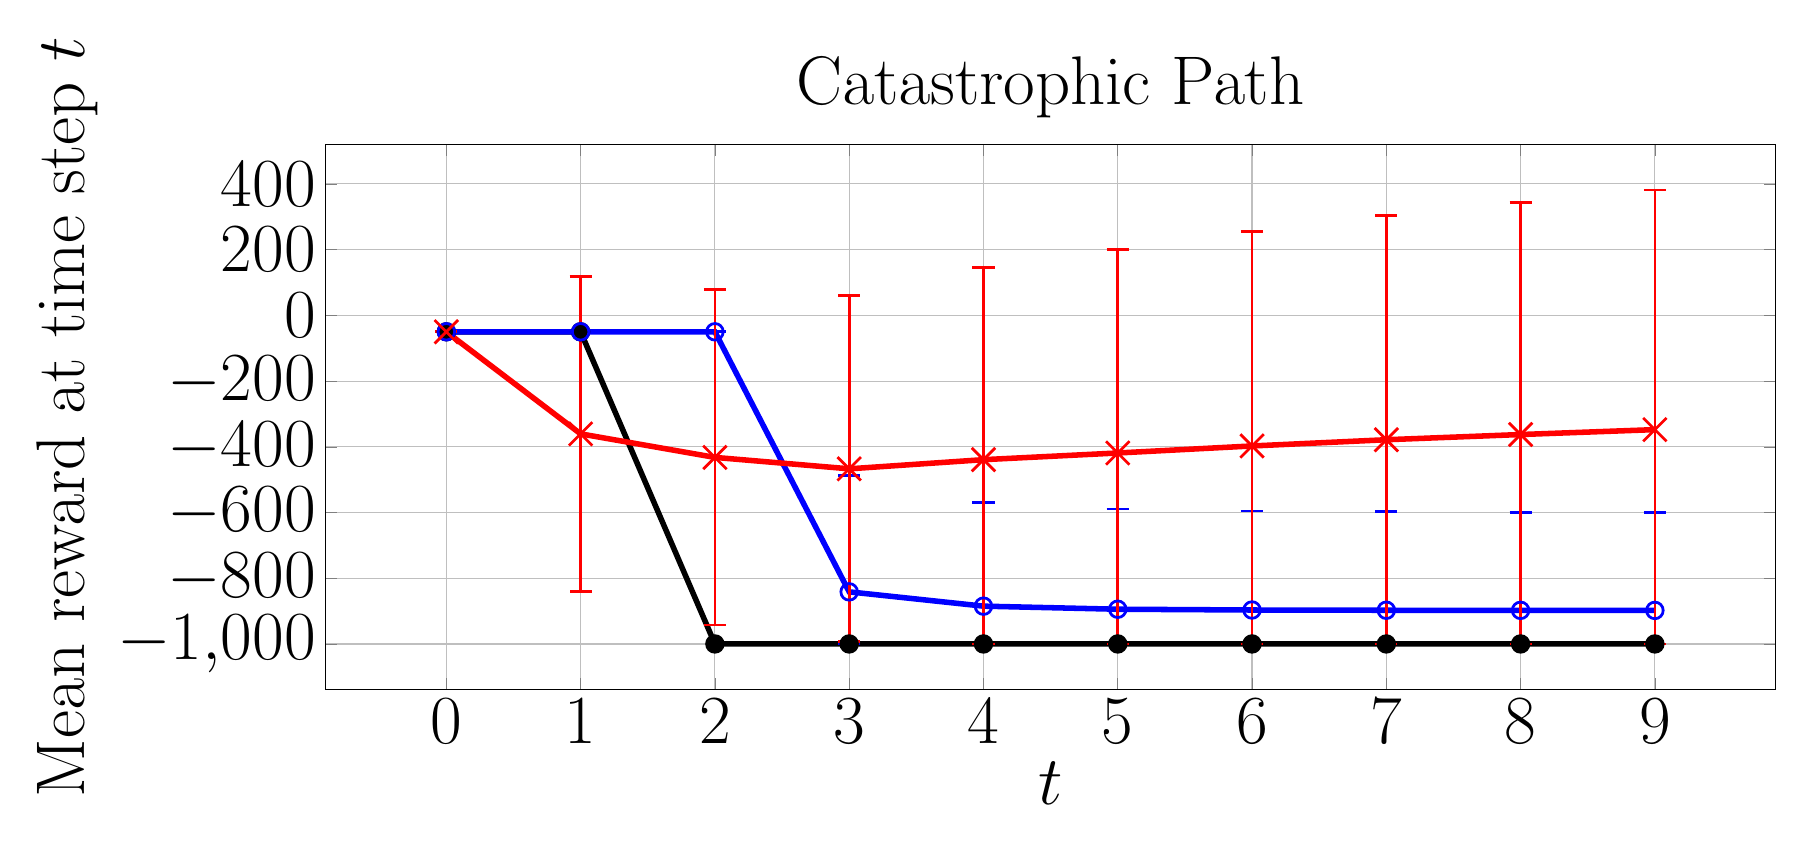
\begin{tikzpicture}
                \begin{axis}[
                    xlabel={$t$},
                    ylabel={Mean reward at time step $t$},
                    title={Catastrophic Path},
                    grid=both,
                    width=20cm, height=8.5cm,
                    every axis/.style={font=\Huge},
                    %
                ]
               \addplot[
                    color=black, %
                    mark=*, %
                    line width=2pt,
                    mark size=3pt,
                ]
                coordinates {
                    (0, -50.0)
                    (1, -50.0)
                    (2, -1000.0)
                    (3, -1000.0)
                    (4, -1000.0)
                    (5, -1000.0)
                    (6, -1000.0)
                    (7, -1000.0)
                    (8, -1000.0)
                    (9, -1000.0)
                };
                %
                %
                \addplot[
                    color=blue, %
                    mark=o, %
                    line width=2pt,
                    mark size=3pt,
                    error bars/.cd,
                    y dir=both, %
                    y explicit, %
                    error bar style={line width=1pt,solid},
                    error mark options={line width=1pt,mark size=4pt,rotate=90}
                ]
                coordinates {
                    (0, -50.0)  +- (0, 0.0)
                    (1, -50.0)  +- (0, 0.0) 
                    (2, -50.0)  +- (0, 0.0) 
                    (3, -841.440725)  += (0, 354.24605512) -= (0, 158.559275)
                    (4, -884.98225)  += (0, 315.37519669) -= (0, 115.01775)
                    (5, -894.330425) += (0, 304.88572805) -= (0, 105.669575)
                    (6, -896.696175) += (0, 301.19954514) -= (0, 103.303825)
                    (7, -897.4635) += (0, 299.61791279) -= (0, 102.5365)
                    (8, -897.77595) += (0, 298.80392585) -= (0, 102.22405)
                    (9, -897.942975) += (0, 298.32920557) -= (0, 102.057025)
                };
                %
                \addplot[
                    color=red, %
                    mark=x, %
                    line width=2pt,
                    mark size=6pt,
                    error bars/.cd,
                    y dir=both, %
                    y explicit, %
                    error bar style={line width=1pt,solid},
                    error mark options={line width=1pt,mark size=4pt,rotate=90}
                ]
            coordinates {
                    (0, -50.0)  +- (0, 0.0)
                    (1, -360.675265)  +- (0, 479.39812699) 
                    (2, -432.27629)  +- (0, 510.38620897) 
                    (3, -467.029545)  += (0, 526.36009628) -= (0, 526.36009628)
                    (4, -439.17429)  += (0, 583.96638919) -= (0, 560.82571)
                    (5, -418.82704) += (0, 618.43027478) -= (0, 581.17296)
                    (6, -397.464895) += (0, 652.67322574) -= (0, 602.535105)
                    (7, -378.49052) += (0, 682.85407033) -= (0, 621.50948)
                    (8, -362.654195) += (0, 707.01412023) -= (0, 637.345805)
                    (9, -347.737935) += (0, 729.29076479) -= (0, 652.262065)
                };
                %
                %
                %
                %
                %
                %
                %
                %
                %
                %
                %
                %
                %
                %
                %
                %
                %
                %
                %
                \end{axis}
            \end{tikzpicture}
         }
    }
    \caption{Average instant reward of CF paths induced by policies on Sepsis.}
    \label{fig: reward sepsis}
\end{figure*}

%
%
%
\subsection{Interval CFMDP Bounds}
%
%
Table \ref{tab:nonzero_probs} presents the mean counterfactual probability bound widths (excluding transitions where the upper bound is $0$) for each MDP, averaged over 20 observed paths. We compare the bounds under counterfactual stability (CS) and monotonicity (M) assumptions, CS alone, and no assumptions. This shows that the assumptions marginally reduce the bound widths, indicating the assumptions tighten the bounds without excluding too many causal models, as intended.
\renewcommand{\arraystretch}{1}

\begin{table}
\centering
\caption{Mean width of counterfactual probability bounds}
\resizebox{0.8\columnwidth}{!}{%
\begin{tabular}{|c|c|c|c|}
\hline
\multirow{2}{*}{\textbf{Environment}} & \multicolumn{3}{c|}{\textbf{Assumptions}} \\ \cline{2-4}
 & \textbf{CS + M} & \textbf{CS} & \textbf{None\tablefootnote{\jl{Equivalent to \citet{li2024probabilities}'s bounds (see Section \ref{sec: equivalence with Li}).}}} \\ \hline
\textbf{GridWorld} ($p=0.9$) & 0.0817 & 0.0977 & 0.100 \\ \hline
\textbf{GridWorld} ($p=0.4$) & 0.552  & 0.638  & 0.646 \\ \hline
\textbf{Sepsis} & 0.138 & 0.140 & 0.140 \\ \hline
\end{tabular}
}
\label{tab:nonzero_probs}
\end{table}


\subsection{Execution Times}
Table \ref{tab: times} compares the average time needed to generate the interval CFMDP vs.\ the Gumbel-max SCM CFMDP for 20 observations.
The GridWorld algorithms were run single-threaded, while the Sepsis experiments were run in parallel.
Generating the interval CFMDP is significantly faster as it uses exact analytical bounds, whereas the Gumbel-max CFMDP requires sampling from the Gumbel distribution to estimate counterfactual transition probabilities. \jl{Since constructing the counterfactual MDP models is the main bottleneck in both approaches, ours is more efficient overall and suitable for larger MDPs.}
\begin{table}
\centering
\caption{Mean execution time to generate CFMDPs}
\resizebox{0.99\columnwidth}{!}{%
\begin{tabular}{|c|c|c|}
\hline
\multirow{2}{*}{\textbf{Environment}} & \multicolumn{2}{c|}{\textbf{Mean Execution Time (s)}} \\ \cline{2-3} 
                                      & \textbf{Interval CFMDP} & \textbf{Gumbel-max CFMDP} \\ \hline
\textbf{GridWorld ($p=0.9$) }                  & 0.261                   & 56.1                      \\ \hline
\textbf{GridWorld ($p=0.4$)  }                 & 0.336                   & 54.5                      \\ \hline
\textbf{Sepsis}                                 & 688                     & 2940                      \\ \hline
\end{tabular}%
}
\label{tab: times}
\end{table}


\section{Conclusion}
In this work, we propose a simple yet effective approach, called SMILE, for graph few-shot learning with fewer tasks. Specifically, we introduce a novel dual-level mixup strategy, including within-task and across-task mixup, for enriching the diversity of nodes within each task and the diversity of tasks. Also, we incorporate the degree-based prior information to learn expressive node embeddings. Theoretically, we prove that SMILE effectively enhances the model's generalization performance. Empirically, we conduct extensive experiments on multiple benchmarks and the results suggest that SMILE significantly outperforms other baselines, including both in-domain and cross-domain few-shot settings.

\begin{acknowledgements}
The authors would like to thank Frederik Mathiesen and 
Luca Laurenti for their support with using the IntervalMDP.jl package. This work was supported by UK Research and Innovation [grant number EP/S023356/1] in the UKRI Centre for Doctoral Training in Safe and Trusted Artificial Intelligence (www.safeandtrustedai.org); and UK Research and Innovation [grant number EP/W014785/2].
\end{acknowledgements}

%
\bibliography{bibliography}

\newpage

\onecolumn

\title{Robust Counterfactual Inference in Markov Decision Processes\\(Supplementary Material)}
\maketitle

\appendix
\subsection{Lloyd-Max Algorithm}
\label{subsec:Lloyd-Max}
For a given quantization bitwidth $B$ and an operand $\bm{X}$, the Lloyd-Max algorithm finds $2^B$ quantization levels $\{\hat{x}_i\}_{i=1}^{2^B}$ such that quantizing $\bm{X}$ by rounding each scalar in $\bm{X}$ to the nearest quantization level minimizes the quantization MSE. 

The algorithm starts with an initial guess of quantization levels and then iteratively computes quantization thresholds $\{\tau_i\}_{i=1}^{2^B-1}$ and updates quantization levels $\{\hat{x}_i\}_{i=1}^{2^B}$. Specifically, at iteration $n$, thresholds are set to the midpoints of the previous iteration's levels:
\begin{align*}
    \tau_i^{(n)}=\frac{\hat{x}_i^{(n-1)}+\hat{x}_{i+1}^{(n-1)}}2 \text{ for } i=1\ldots 2^B-1
\end{align*}
Subsequently, the quantization levels are re-computed as conditional means of the data regions defined by the new thresholds:
\begin{align*}
    \hat{x}_i^{(n)}=\mathbb{E}\left[ \bm{X} \big| \bm{X}\in [\tau_{i-1}^{(n)},\tau_i^{(n)}] \right] \text{ for } i=1\ldots 2^B
\end{align*}
where to satisfy boundary conditions we have $\tau_0=-\infty$ and $\tau_{2^B}=\infty$. The algorithm iterates the above steps until convergence.

Figure \ref{fig:lm_quant} compares the quantization levels of a $7$-bit floating point (E3M3) quantizer (left) to a $7$-bit Lloyd-Max quantizer (right) when quantizing a layer of weights from the GPT3-126M model at a per-tensor granularity. As shown, the Lloyd-Max quantizer achieves substantially lower quantization MSE. Further, Table \ref{tab:FP7_vs_LM7} shows the superior perplexity achieved by Lloyd-Max quantizers for bitwidths of $7$, $6$ and $5$. The difference between the quantizers is clear at 5 bits, where per-tensor FP quantization incurs a drastic and unacceptable increase in perplexity, while Lloyd-Max quantization incurs a much smaller increase. Nevertheless, we note that even the optimal Lloyd-Max quantizer incurs a notable ($\sim 1.5$) increase in perplexity due to the coarse granularity of quantization. 

\begin{figure}[h]
  \centering
  \includegraphics[width=0.7\linewidth]{sections/figures/LM7_FP7.pdf}
  \caption{\small Quantization levels and the corresponding quantization MSE of Floating Point (left) vs Lloyd-Max (right) Quantizers for a layer of weights in the GPT3-126M model.}
  \label{fig:lm_quant}
\end{figure}

\begin{table}[h]\scriptsize
\begin{center}
\caption{\label{tab:FP7_vs_LM7} \small Comparing perplexity (lower is better) achieved by floating point quantizers and Lloyd-Max quantizers on a GPT3-126M model for the Wikitext-103 dataset.}
\begin{tabular}{c|cc|c}
\hline
 \multirow{2}{*}{\textbf{Bitwidth}} & \multicolumn{2}{|c|}{\textbf{Floating-Point Quantizer}} & \textbf{Lloyd-Max Quantizer} \\
 & Best Format & Wikitext-103 Perplexity & Wikitext-103 Perplexity \\
\hline
7 & E3M3 & 18.32 & 18.27 \\
6 & E3M2 & 19.07 & 18.51 \\
5 & E4M0 & 43.89 & 19.71 \\
\hline
\end{tabular}
\end{center}
\end{table}

\subsection{Proof of Local Optimality of LO-BCQ}
\label{subsec:lobcq_opt_proof}
For a given block $\bm{b}_j$, the quantization MSE during LO-BCQ can be empirically evaluated as $\frac{1}{L_b}\lVert \bm{b}_j- \bm{\hat{b}}_j\rVert^2_2$ where $\bm{\hat{b}}_j$ is computed from equation (\ref{eq:clustered_quantization_definition}) as $C_{f(\bm{b}_j)}(\bm{b}_j)$. Further, for a given block cluster $\mathcal{B}_i$, we compute the quantization MSE as $\frac{1}{|\mathcal{B}_{i}|}\sum_{\bm{b} \in \mathcal{B}_{i}} \frac{1}{L_b}\lVert \bm{b}- C_i^{(n)}(\bm{b})\rVert^2_2$. Therefore, at the end of iteration $n$, we evaluate the overall quantization MSE $J^{(n)}$ for a given operand $\bm{X}$ composed of $N_c$ block clusters as:
\begin{align*}
    \label{eq:mse_iter_n}
    J^{(n)} = \frac{1}{N_c} \sum_{i=1}^{N_c} \frac{1}{|\mathcal{B}_{i}^{(n)}|}\sum_{\bm{v} \in \mathcal{B}_{i}^{(n)}} \frac{1}{L_b}\lVert \bm{b}- B_i^{(n)}(\bm{b})\rVert^2_2
\end{align*}

At the end of iteration $n$, the codebooks are updated from $\mathcal{C}^{(n-1)}$ to $\mathcal{C}^{(n)}$. However, the mapping of a given vector $\bm{b}_j$ to quantizers $\mathcal{C}^{(n)}$ remains as  $f^{(n)}(\bm{b}_j)$. At the next iteration, during the vector clustering step, $f^{(n+1)}(\bm{b}_j)$ finds new mapping of $\bm{b}_j$ to updated codebooks $\mathcal{C}^{(n)}$ such that the quantization MSE over the candidate codebooks is minimized. Therefore, we obtain the following result for $\bm{b}_j$:
\begin{align*}
\frac{1}{L_b}\lVert \bm{b}_j - C_{f^{(n+1)}(\bm{b}_j)}^{(n)}(\bm{b}_j)\rVert^2_2 \le \frac{1}{L_b}\lVert \bm{b}_j - C_{f^{(n)}(\bm{b}_j)}^{(n)}(\bm{b}_j)\rVert^2_2
\end{align*}

That is, quantizing $\bm{b}_j$ at the end of the block clustering step of iteration $n+1$ results in lower quantization MSE compared to quantizing at the end of iteration $n$. Since this is true for all $\bm{b} \in \bm{X}$, we assert the following:
\begin{equation}
\begin{split}
\label{eq:mse_ineq_1}
    \tilde{J}^{(n+1)} &= \frac{1}{N_c} \sum_{i=1}^{N_c} \frac{1}{|\mathcal{B}_{i}^{(n+1)}|}\sum_{\bm{b} \in \mathcal{B}_{i}^{(n+1)}} \frac{1}{L_b}\lVert \bm{b} - C_i^{(n)}(b)\rVert^2_2 \le J^{(n)}
\end{split}
\end{equation}
where $\tilde{J}^{(n+1)}$ is the the quantization MSE after the vector clustering step at iteration $n+1$.

Next, during the codebook update step (\ref{eq:quantizers_update}) at iteration $n+1$, the per-cluster codebooks $\mathcal{C}^{(n)}$ are updated to $\mathcal{C}^{(n+1)}$ by invoking the Lloyd-Max algorithm \citep{Lloyd}. We know that for any given value distribution, the Lloyd-Max algorithm minimizes the quantization MSE. Therefore, for a given vector cluster $\mathcal{B}_i$ we obtain the following result:

\begin{equation}
    \frac{1}{|\mathcal{B}_{i}^{(n+1)}|}\sum_{\bm{b} \in \mathcal{B}_{i}^{(n+1)}} \frac{1}{L_b}\lVert \bm{b}- C_i^{(n+1)}(\bm{b})\rVert^2_2 \le \frac{1}{|\mathcal{B}_{i}^{(n+1)}|}\sum_{\bm{b} \in \mathcal{B}_{i}^{(n+1)}} \frac{1}{L_b}\lVert \bm{b}- C_i^{(n)}(\bm{b})\rVert^2_2
\end{equation}

The above equation states that quantizing the given block cluster $\mathcal{B}_i$ after updating the associated codebook from $C_i^{(n)}$ to $C_i^{(n+1)}$ results in lower quantization MSE. Since this is true for all the block clusters, we derive the following result: 
\begin{equation}
\begin{split}
\label{eq:mse_ineq_2}
     J^{(n+1)} &= \frac{1}{N_c} \sum_{i=1}^{N_c} \frac{1}{|\mathcal{B}_{i}^{(n+1)}|}\sum_{\bm{b} \in \mathcal{B}_{i}^{(n+1)}} \frac{1}{L_b}\lVert \bm{b}- C_i^{(n+1)}(\bm{b})\rVert^2_2  \le \tilde{J}^{(n+1)}   
\end{split}
\end{equation}

Following (\ref{eq:mse_ineq_1}) and (\ref{eq:mse_ineq_2}), we find that the quantization MSE is non-increasing for each iteration, that is, $J^{(1)} \ge J^{(2)} \ge J^{(3)} \ge \ldots \ge J^{(M)}$ where $M$ is the maximum number of iterations. 
%Therefore, we can say that if the algorithm converges, then it must be that it has converged to a local minimum. 
\hfill $\blacksquare$


\begin{figure}
    \begin{center}
    \includegraphics[width=0.5\textwidth]{sections//figures/mse_vs_iter.pdf}
    \end{center}
    \caption{\small NMSE vs iterations during LO-BCQ compared to other block quantization proposals}
    \label{fig:nmse_vs_iter}
\end{figure}

Figure \ref{fig:nmse_vs_iter} shows the empirical convergence of LO-BCQ across several block lengths and number of codebooks. Also, the MSE achieved by LO-BCQ is compared to baselines such as MXFP and VSQ. As shown, LO-BCQ converges to a lower MSE than the baselines. Further, we achieve better convergence for larger number of codebooks ($N_c$) and for a smaller block length ($L_b$), both of which increase the bitwidth of BCQ (see Eq \ref{eq:bitwidth_bcq}).


\subsection{Additional Accuracy Results}
%Table \ref{tab:lobcq_config} lists the various LOBCQ configurations and their corresponding bitwidths.
\begin{table}
\setlength{\tabcolsep}{4.75pt}
\begin{center}
\caption{\label{tab:lobcq_config} Various LO-BCQ configurations and their bitwidths.}
\begin{tabular}{|c||c|c|c|c||c|c||c|} 
\hline
 & \multicolumn{4}{|c||}{$L_b=8$} & \multicolumn{2}{|c||}{$L_b=4$} & $L_b=2$ \\
 \hline
 \backslashbox{$L_A$\kern-1em}{\kern-1em$N_c$} & 2 & 4 & 8 & 16 & 2 & 4 & 2 \\
 \hline
 64 & 4.25 & 4.375 & 4.5 & 4.625 & 4.375 & 4.625 & 4.625\\
 \hline
 32 & 4.375 & 4.5 & 4.625& 4.75 & 4.5 & 4.75 & 4.75 \\
 \hline
 16 & 4.625 & 4.75& 4.875 & 5 & 4.75 & 5 & 5 \\
 \hline
\end{tabular}
\end{center}
\end{table}

%\subsection{Perplexity achieved by various LO-BCQ configurations on Wikitext-103 dataset}

\begin{table} \centering
\begin{tabular}{|c||c|c|c|c||c|c||c|} 
\hline
 $L_b \rightarrow$& \multicolumn{4}{c||}{8} & \multicolumn{2}{c||}{4} & 2\\
 \hline
 \backslashbox{$L_A$\kern-1em}{\kern-1em$N_c$} & 2 & 4 & 8 & 16 & 2 & 4 & 2  \\
 %$N_c \rightarrow$ & 2 & 4 & 8 & 16 & 2 & 4 & 2 \\
 \hline
 \hline
 \multicolumn{8}{c}{GPT3-1.3B (FP32 PPL = 9.98)} \\ 
 \hline
 \hline
 64 & 10.40 & 10.23 & 10.17 & 10.15 &  10.28 & 10.18 & 10.19 \\
 \hline
 32 & 10.25 & 10.20 & 10.15 & 10.12 &  10.23 & 10.17 & 10.17 \\
 \hline
 16 & 10.22 & 10.16 & 10.10 & 10.09 &  10.21 & 10.14 & 10.16 \\
 \hline
  \hline
 \multicolumn{8}{c}{GPT3-8B (FP32 PPL = 7.38)} \\ 
 \hline
 \hline
 64 & 7.61 & 7.52 & 7.48 &  7.47 &  7.55 &  7.49 & 7.50 \\
 \hline
 32 & 7.52 & 7.50 & 7.46 &  7.45 &  7.52 &  7.48 & 7.48  \\
 \hline
 16 & 7.51 & 7.48 & 7.44 &  7.44 &  7.51 &  7.49 & 7.47  \\
 \hline
\end{tabular}
\caption{\label{tab:ppl_gpt3_abalation} Wikitext-103 perplexity across GPT3-1.3B and 8B models.}
\end{table}

\begin{table} \centering
\begin{tabular}{|c||c|c|c|c||} 
\hline
 $L_b \rightarrow$& \multicolumn{4}{c||}{8}\\
 \hline
 \backslashbox{$L_A$\kern-1em}{\kern-1em$N_c$} & 2 & 4 & 8 & 16 \\
 %$N_c \rightarrow$ & 2 & 4 & 8 & 16 & 2 & 4 & 2 \\
 \hline
 \hline
 \multicolumn{5}{|c|}{Llama2-7B (FP32 PPL = 5.06)} \\ 
 \hline
 \hline
 64 & 5.31 & 5.26 & 5.19 & 5.18  \\
 \hline
 32 & 5.23 & 5.25 & 5.18 & 5.15  \\
 \hline
 16 & 5.23 & 5.19 & 5.16 & 5.14  \\
 \hline
 \multicolumn{5}{|c|}{Nemotron4-15B (FP32 PPL = 5.87)} \\ 
 \hline
 \hline
 64  & 6.3 & 6.20 & 6.13 & 6.08  \\
 \hline
 32  & 6.24 & 6.12 & 6.07 & 6.03  \\
 \hline
 16  & 6.12 & 6.14 & 6.04 & 6.02  \\
 \hline
 \multicolumn{5}{|c|}{Nemotron4-340B (FP32 PPL = 3.48)} \\ 
 \hline
 \hline
 64 & 3.67 & 3.62 & 3.60 & 3.59 \\
 \hline
 32 & 3.63 & 3.61 & 3.59 & 3.56 \\
 \hline
 16 & 3.61 & 3.58 & 3.57 & 3.55 \\
 \hline
\end{tabular}
\caption{\label{tab:ppl_llama7B_nemo15B} Wikitext-103 perplexity compared to FP32 baseline in Llama2-7B and Nemotron4-15B, 340B models}
\end{table}

%\subsection{Perplexity achieved by various LO-BCQ configurations on MMLU dataset}


\begin{table} \centering
\begin{tabular}{|c||c|c|c|c||c|c|c|c|} 
\hline
 $L_b \rightarrow$& \multicolumn{4}{c||}{8} & \multicolumn{4}{c||}{8}\\
 \hline
 \backslashbox{$L_A$\kern-1em}{\kern-1em$N_c$} & 2 & 4 & 8 & 16 & 2 & 4 & 8 & 16  \\
 %$N_c \rightarrow$ & 2 & 4 & 8 & 16 & 2 & 4 & 2 \\
 \hline
 \hline
 \multicolumn{5}{|c|}{Llama2-7B (FP32 Accuracy = 45.8\%)} & \multicolumn{4}{|c|}{Llama2-70B (FP32 Accuracy = 69.12\%)} \\ 
 \hline
 \hline
 64 & 43.9 & 43.4 & 43.9 & 44.9 & 68.07 & 68.27 & 68.17 & 68.75 \\
 \hline
 32 & 44.5 & 43.8 & 44.9 & 44.5 & 68.37 & 68.51 & 68.35 & 68.27  \\
 \hline
 16 & 43.9 & 42.7 & 44.9 & 45 & 68.12 & 68.77 & 68.31 & 68.59  \\
 \hline
 \hline
 \multicolumn{5}{|c|}{GPT3-22B (FP32 Accuracy = 38.75\%)} & \multicolumn{4}{|c|}{Nemotron4-15B (FP32 Accuracy = 64.3\%)} \\ 
 \hline
 \hline
 64 & 36.71 & 38.85 & 38.13 & 38.92 & 63.17 & 62.36 & 63.72 & 64.09 \\
 \hline
 32 & 37.95 & 38.69 & 39.45 & 38.34 & 64.05 & 62.30 & 63.8 & 64.33  \\
 \hline
 16 & 38.88 & 38.80 & 38.31 & 38.92 & 63.22 & 63.51 & 63.93 & 64.43  \\
 \hline
\end{tabular}
\caption{\label{tab:mmlu_abalation} Accuracy on MMLU dataset across GPT3-22B, Llama2-7B, 70B and Nemotron4-15B models.}
\end{table}


%\subsection{Perplexity achieved by various LO-BCQ configurations on LM evaluation harness}

\begin{table} \centering
\begin{tabular}{|c||c|c|c|c||c|c|c|c|} 
\hline
 $L_b \rightarrow$& \multicolumn{4}{c||}{8} & \multicolumn{4}{c||}{8}\\
 \hline
 \backslashbox{$L_A$\kern-1em}{\kern-1em$N_c$} & 2 & 4 & 8 & 16 & 2 & 4 & 8 & 16  \\
 %$N_c \rightarrow$ & 2 & 4 & 8 & 16 & 2 & 4 & 2 \\
 \hline
 \hline
 \multicolumn{5}{|c|}{Race (FP32 Accuracy = 37.51\%)} & \multicolumn{4}{|c|}{Boolq (FP32 Accuracy = 64.62\%)} \\ 
 \hline
 \hline
 64 & 36.94 & 37.13 & 36.27 & 37.13 & 63.73 & 62.26 & 63.49 & 63.36 \\
 \hline
 32 & 37.03 & 36.36 & 36.08 & 37.03 & 62.54 & 63.51 & 63.49 & 63.55  \\
 \hline
 16 & 37.03 & 37.03 & 36.46 & 37.03 & 61.1 & 63.79 & 63.58 & 63.33  \\
 \hline
 \hline
 \multicolumn{5}{|c|}{Winogrande (FP32 Accuracy = 58.01\%)} & \multicolumn{4}{|c|}{Piqa (FP32 Accuracy = 74.21\%)} \\ 
 \hline
 \hline
 64 & 58.17 & 57.22 & 57.85 & 58.33 & 73.01 & 73.07 & 73.07 & 72.80 \\
 \hline
 32 & 59.12 & 58.09 & 57.85 & 58.41 & 73.01 & 73.94 & 72.74 & 73.18  \\
 \hline
 16 & 57.93 & 58.88 & 57.93 & 58.56 & 73.94 & 72.80 & 73.01 & 73.94  \\
 \hline
\end{tabular}
\caption{\label{tab:mmlu_abalation} Accuracy on LM evaluation harness tasks on GPT3-1.3B model.}
\end{table}

\begin{table} \centering
\begin{tabular}{|c||c|c|c|c||c|c|c|c|} 
\hline
 $L_b \rightarrow$& \multicolumn{4}{c||}{8} & \multicolumn{4}{c||}{8}\\
 \hline
 \backslashbox{$L_A$\kern-1em}{\kern-1em$N_c$} & 2 & 4 & 8 & 16 & 2 & 4 & 8 & 16  \\
 %$N_c \rightarrow$ & 2 & 4 & 8 & 16 & 2 & 4 & 2 \\
 \hline
 \hline
 \multicolumn{5}{|c|}{Race (FP32 Accuracy = 41.34\%)} & \multicolumn{4}{|c|}{Boolq (FP32 Accuracy = 68.32\%)} \\ 
 \hline
 \hline
 64 & 40.48 & 40.10 & 39.43 & 39.90 & 69.20 & 68.41 & 69.45 & 68.56 \\
 \hline
 32 & 39.52 & 39.52 & 40.77 & 39.62 & 68.32 & 67.43 & 68.17 & 69.30  \\
 \hline
 16 & 39.81 & 39.71 & 39.90 & 40.38 & 68.10 & 66.33 & 69.51 & 69.42  \\
 \hline
 \hline
 \multicolumn{5}{|c|}{Winogrande (FP32 Accuracy = 67.88\%)} & \multicolumn{4}{|c|}{Piqa (FP32 Accuracy = 78.78\%)} \\ 
 \hline
 \hline
 64 & 66.85 & 66.61 & 67.72 & 67.88 & 77.31 & 77.42 & 77.75 & 77.64 \\
 \hline
 32 & 67.25 & 67.72 & 67.72 & 67.00 & 77.31 & 77.04 & 77.80 & 77.37  \\
 \hline
 16 & 68.11 & 68.90 & 67.88 & 67.48 & 77.37 & 78.13 & 78.13 & 77.69  \\
 \hline
\end{tabular}
\caption{\label{tab:mmlu_abalation} Accuracy on LM evaluation harness tasks on GPT3-8B model.}
\end{table}

\begin{table} \centering
\begin{tabular}{|c||c|c|c|c||c|c|c|c|} 
\hline
 $L_b \rightarrow$& \multicolumn{4}{c||}{8} & \multicolumn{4}{c||}{8}\\
 \hline
 \backslashbox{$L_A$\kern-1em}{\kern-1em$N_c$} & 2 & 4 & 8 & 16 & 2 & 4 & 8 & 16  \\
 %$N_c \rightarrow$ & 2 & 4 & 8 & 16 & 2 & 4 & 2 \\
 \hline
 \hline
 \multicolumn{5}{|c|}{Race (FP32 Accuracy = 40.67\%)} & \multicolumn{4}{|c|}{Boolq (FP32 Accuracy = 76.54\%)} \\ 
 \hline
 \hline
 64 & 40.48 & 40.10 & 39.43 & 39.90 & 75.41 & 75.11 & 77.09 & 75.66 \\
 \hline
 32 & 39.52 & 39.52 & 40.77 & 39.62 & 76.02 & 76.02 & 75.96 & 75.35  \\
 \hline
 16 & 39.81 & 39.71 & 39.90 & 40.38 & 75.05 & 73.82 & 75.72 & 76.09  \\
 \hline
 \hline
 \multicolumn{5}{|c|}{Winogrande (FP32 Accuracy = 70.64\%)} & \multicolumn{4}{|c|}{Piqa (FP32 Accuracy = 79.16\%)} \\ 
 \hline
 \hline
 64 & 69.14 & 70.17 & 70.17 & 70.56 & 78.24 & 79.00 & 78.62 & 78.73 \\
 \hline
 32 & 70.96 & 69.69 & 71.27 & 69.30 & 78.56 & 79.49 & 79.16 & 78.89  \\
 \hline
 16 & 71.03 & 69.53 & 69.69 & 70.40 & 78.13 & 79.16 & 79.00 & 79.00  \\
 \hline
\end{tabular}
\caption{\label{tab:mmlu_abalation} Accuracy on LM evaluation harness tasks on GPT3-22B model.}
\end{table}

\begin{table} \centering
\begin{tabular}{|c||c|c|c|c||c|c|c|c|} 
\hline
 $L_b \rightarrow$& \multicolumn{4}{c||}{8} & \multicolumn{4}{c||}{8}\\
 \hline
 \backslashbox{$L_A$\kern-1em}{\kern-1em$N_c$} & 2 & 4 & 8 & 16 & 2 & 4 & 8 & 16  \\
 %$N_c \rightarrow$ & 2 & 4 & 8 & 16 & 2 & 4 & 2 \\
 \hline
 \hline
 \multicolumn{5}{|c|}{Race (FP32 Accuracy = 44.4\%)} & \multicolumn{4}{|c|}{Boolq (FP32 Accuracy = 79.29\%)} \\ 
 \hline
 \hline
 64 & 42.49 & 42.51 & 42.58 & 43.45 & 77.58 & 77.37 & 77.43 & 78.1 \\
 \hline
 32 & 43.35 & 42.49 & 43.64 & 43.73 & 77.86 & 75.32 & 77.28 & 77.86  \\
 \hline
 16 & 44.21 & 44.21 & 43.64 & 42.97 & 78.65 & 77 & 76.94 & 77.98  \\
 \hline
 \hline
 \multicolumn{5}{|c|}{Winogrande (FP32 Accuracy = 69.38\%)} & \multicolumn{4}{|c|}{Piqa (FP32 Accuracy = 78.07\%)} \\ 
 \hline
 \hline
 64 & 68.9 & 68.43 & 69.77 & 68.19 & 77.09 & 76.82 & 77.09 & 77.86 \\
 \hline
 32 & 69.38 & 68.51 & 68.82 & 68.90 & 78.07 & 76.71 & 78.07 & 77.86  \\
 \hline
 16 & 69.53 & 67.09 & 69.38 & 68.90 & 77.37 & 77.8 & 77.91 & 77.69  \\
 \hline
\end{tabular}
\caption{\label{tab:mmlu_abalation} Accuracy on LM evaluation harness tasks on Llama2-7B model.}
\end{table}

\begin{table} \centering
\begin{tabular}{|c||c|c|c|c||c|c|c|c|} 
\hline
 $L_b \rightarrow$& \multicolumn{4}{c||}{8} & \multicolumn{4}{c||}{8}\\
 \hline
 \backslashbox{$L_A$\kern-1em}{\kern-1em$N_c$} & 2 & 4 & 8 & 16 & 2 & 4 & 8 & 16  \\
 %$N_c \rightarrow$ & 2 & 4 & 8 & 16 & 2 & 4 & 2 \\
 \hline
 \hline
 \multicolumn{5}{|c|}{Race (FP32 Accuracy = 48.8\%)} & \multicolumn{4}{|c|}{Boolq (FP32 Accuracy = 85.23\%)} \\ 
 \hline
 \hline
 64 & 49.00 & 49.00 & 49.28 & 48.71 & 82.82 & 84.28 & 84.03 & 84.25 \\
 \hline
 32 & 49.57 & 48.52 & 48.33 & 49.28 & 83.85 & 84.46 & 84.31 & 84.93  \\
 \hline
 16 & 49.85 & 49.09 & 49.28 & 48.99 & 85.11 & 84.46 & 84.61 & 83.94  \\
 \hline
 \hline
 \multicolumn{5}{|c|}{Winogrande (FP32 Accuracy = 79.95\%)} & \multicolumn{4}{|c|}{Piqa (FP32 Accuracy = 81.56\%)} \\ 
 \hline
 \hline
 64 & 78.77 & 78.45 & 78.37 & 79.16 & 81.45 & 80.69 & 81.45 & 81.5 \\
 \hline
 32 & 78.45 & 79.01 & 78.69 & 80.66 & 81.56 & 80.58 & 81.18 & 81.34  \\
 \hline
 16 & 79.95 & 79.56 & 79.79 & 79.72 & 81.28 & 81.66 & 81.28 & 80.96  \\
 \hline
\end{tabular}
\caption{\label{tab:mmlu_abalation} Accuracy on LM evaluation harness tasks on Llama2-70B model.}
\end{table}

%\section{MSE Studies}
%\textcolor{red}{TODO}


\subsection{Number Formats and Quantization Method}
\label{subsec:numFormats_quantMethod}
\subsubsection{Integer Format}
An $n$-bit signed integer (INT) is typically represented with a 2s-complement format \citep{yao2022zeroquant,xiao2023smoothquant,dai2021vsq}, where the most significant bit denotes the sign.

\subsubsection{Floating Point Format}
An $n$-bit signed floating point (FP) number $x$ comprises of a 1-bit sign ($x_{\mathrm{sign}}$), $B_m$-bit mantissa ($x_{\mathrm{mant}}$) and $B_e$-bit exponent ($x_{\mathrm{exp}}$) such that $B_m+B_e=n-1$. The associated constant exponent bias ($E_{\mathrm{bias}}$) is computed as $(2^{{B_e}-1}-1)$. We denote this format as $E_{B_e}M_{B_m}$.  

\subsubsection{Quantization Scheme}
\label{subsec:quant_method}
A quantization scheme dictates how a given unquantized tensor is converted to its quantized representation. We consider FP formats for the purpose of illustration. Given an unquantized tensor $\bm{X}$ and an FP format $E_{B_e}M_{B_m}$, we first, we compute the quantization scale factor $s_X$ that maps the maximum absolute value of $\bm{X}$ to the maximum quantization level of the $E_{B_e}M_{B_m}$ format as follows:
\begin{align}
\label{eq:sf}
    s_X = \frac{\mathrm{max}(|\bm{X}|)}{\mathrm{max}(E_{B_e}M_{B_m})}
\end{align}
In the above equation, $|\cdot|$ denotes the absolute value function.

Next, we scale $\bm{X}$ by $s_X$ and quantize it to $\hat{\bm{X}}$ by rounding it to the nearest quantization level of $E_{B_e}M_{B_m}$ as:

\begin{align}
\label{eq:tensor_quant}
    \hat{\bm{X}} = \text{round-to-nearest}\left(\frac{\bm{X}}{s_X}, E_{B_e}M_{B_m}\right)
\end{align}

We perform dynamic max-scaled quantization \citep{wu2020integer}, where the scale factor $s$ for activations is dynamically computed during runtime.

\subsection{Vector Scaled Quantization}
\begin{wrapfigure}{r}{0.35\linewidth}
  \centering
  \includegraphics[width=\linewidth]{sections/figures/vsquant.jpg}
  \caption{\small Vectorwise decomposition for per-vector scaled quantization (VSQ \citep{dai2021vsq}).}
  \label{fig:vsquant}
\end{wrapfigure}
During VSQ \citep{dai2021vsq}, the operand tensors are decomposed into 1D vectors in a hardware friendly manner as shown in Figure \ref{fig:vsquant}. Since the decomposed tensors are used as operands in matrix multiplications during inference, it is beneficial to perform this decomposition along the reduction dimension of the multiplication. The vectorwise quantization is performed similar to tensorwise quantization described in Equations \ref{eq:sf} and \ref{eq:tensor_quant}, where a scale factor $s_v$ is required for each vector $\bm{v}$ that maps the maximum absolute value of that vector to the maximum quantization level. While smaller vector lengths can lead to larger accuracy gains, the associated memory and computational overheads due to the per-vector scale factors increases. To alleviate these overheads, VSQ \citep{dai2021vsq} proposed a second level quantization of the per-vector scale factors to unsigned integers, while MX \citep{rouhani2023shared} quantizes them to integer powers of 2 (denoted as $2^{INT}$).

\subsubsection{MX Format}
The MX format proposed in \citep{rouhani2023microscaling} introduces the concept of sub-block shifting. For every two scalar elements of $b$-bits each, there is a shared exponent bit. The value of this exponent bit is determined through an empirical analysis that targets minimizing quantization MSE. We note that the FP format $E_{1}M_{b}$ is strictly better than MX from an accuracy perspective since it allocates a dedicated exponent bit to each scalar as opposed to sharing it across two scalars. Therefore, we conservatively bound the accuracy of a $b+2$-bit signed MX format with that of a $E_{1}M_{b}$ format in our comparisons. For instance, we use E1M2 format as a proxy for MX4.

\begin{figure}
    \centering
    \includegraphics[width=1\linewidth]{sections//figures/BlockFormats.pdf}
    \caption{\small Comparing LO-BCQ to MX format.}
    \label{fig:block_formats}
\end{figure}

Figure \ref{fig:block_formats} compares our $4$-bit LO-BCQ block format to MX \citep{rouhani2023microscaling}. As shown, both LO-BCQ and MX decompose a given operand tensor into block arrays and each block array into blocks. Similar to MX, we find that per-block quantization ($L_b < L_A$) leads to better accuracy due to increased flexibility. While MX achieves this through per-block $1$-bit micro-scales, we associate a dedicated codebook to each block through a per-block codebook selector. Further, MX quantizes the per-block array scale-factor to E8M0 format without per-tensor scaling. In contrast during LO-BCQ, we find that per-tensor scaling combined with quantization of per-block array scale-factor to E4M3 format results in superior inference accuracy across models. 


\end{document}
